\RequirePackage{pdfmanagement}
\SetKeys[document/metadata]{
    pdfversion=2.0, 
    pdfstandard=A-2u,
    lang=pl-PL
}

\documentclass[
    fontsize=12pt,
    paper=a4,
    oneside,
    titlepage=true,
    headinclude=true,
    footinclude=false,
    BCOR=5mm, 
    DIV=11,
    parskip=half,
    numbers=endperiod,
    listof=totoc,
    index=totoc,
    bibliography=totoc,
    abstract=on,
    captions=signature,
]{scrreprt}

\usepackage{preamble}


\newcommand{\myref}[2][rysunku]{%
    \hyperref[#2]{\textsb{#1~\ref{#2}}}%
}

\titlehead{
    \begin{center}
        \sffamily\bfseries\large POLITECHNIKA WARSZAWSKA\\
        \small Wydział Elektryczny
    \end{center}
    \vspace{10mm}
}

\subject{PROJEKT ZESPOŁOWY}
\title{System czasu rzeczywistego detekcji zachowań osób na strumieniach danych z monitoringu wizyjnego}
\subtitle{Dokumentacja Techniczna i Raport Końcowy}
\author{
    \begin{tabular}{ccc}
        \textbf{Mateusz Ciurzyński} & \textbf{Norbert Gwiazda} & \textbf{Bartosz Piłat} \\
        331676 & 331694 & 331727 \\[1.5em]
    \end{tabular}
    \\[0.5em]
    \begin{tabular}{cc}
        \textbf{Borys Piątek} & \textbf{Filip Kobus} \\
        331725 & 331703 \\
    \end{tabular}
}

\date{
    \vspace{10mm}
    {\large Opiekun projektu:}\\[0.5em]
    {\large\bfseries dr\ hab.\ inż.\ Marcin\ Iwanowski}\\[4pt]
    \vfill
    \today
}
\begin{document}

\maketitle

\begin{abstract}
W ramach projektu zaprojektowano i zaimplementowano system czasu rzeczywistego przeznaczony do detekcji zachowań osób na strumieniach danych z monitoringu wizyjnego, przystosowany do integracji z infrastrukturą kamer Politechniki Warszawskiej. Rozwiązanie oparto na potokowym przetwarzaniu obrazu na żywo w oparciu o konfigurowalne szablony detekcji, które precyzują kombinację oraz liczbę obiektów lub zachowań inicjujących rejestrację zdarzenia. 

Moduł detekcji zaimplementowano w języku Python z wykorzystaniem modeli uczenia maszynowego rozpoznających 9 klas obiektów (w tym ludzi, pojazdy i niebezpieczne narzędzia) oraz 7 typów zachowań (m.in.\ upadki, bieg czy wkroczenie w strefę zakazaną). Wdrożono algorytm izolowania fragmentów wideo z buforem czasowym, który zintegrowano z modułem automatycznej anonimizacji twarzy oraz tablic rejestracyjnych. Podsystem zarządzania danymi zrealizowano poprzez ciągły zapis kilkusekundowych segmentów wideo powiązanych w bazie danych strukturą listy jednokierunkowej, co zminimalizowało opóźnienia zapisu dyskowego i umożliwiło wydajne odtwarzanie ciągłego materiału za pomocą protokołu strumieniowania DASH.

Testy systemu przeprowadzono na nagraniach symulujących docelowe otoczenie kampusu uczelni. Poczynione obserwacje wykazały skuteczność potokowej architektury danych oraz zdefiniowały kierunek dalszego rozwoju projektu w stronę implementacji przetwarzania równoległego dla jednoczesnej obsługi wielu kamer.
\end{abstract}

\clearpage
\tableofcontents                
\clearpage


\chapter{Wstęp}
\section{Wprowadzenie do tematyki}
Systemy monitoringu wizyjnego (CCTV) stanowią obecnie kluczowy element utrzymywania bezpieczeństwa w miastach. Większość systemów monitoringowych polega na zapisie pełnego strumienia wideo w celu późniejszej ewentualnej analizy, w przypadku wystąpienia jakiegoś incydentu. Z biegiem lat i wraz ze wzrostem liczby instalowanych kamer, takie podejście staje się coraz trudniejsze, ze względu na czasochłonność ewentualnej analizy wideo z wielu perspektyw.

Przełomem w tej dziedzinie stał się rozwój algorytmów sztucznej inteligencji, a w szczególności ich wykorzystania w widzeniu komputerowym (ang. \textit{Computer Vision}). Współczesne systemy analityki wideo potrafią w czasie rzeczywistym klasyfikować obiekty, śledzić ich ruch i rozpoznawać anomalie. W tę właśnie dziedzinę wpisuje się tematyka niniejszego projektu, którego celem jest przeniesienie problemu detekcji niebezpiecznych lub nietypowych zachowań z człowieka na zautomatyzowany system działający bezpośrednio na strumieniach wideo w czasie rzeczywistym.


\section{Analiza problematyki}
Pomimo powszechności systemów kamer, klasyczne podejście do monitoringu napotyka na szereg istotnych ograniczeń natury ludzkiej, prawnej oraz technologicznej. Projekt rozwiązuje te problemy z następujących obszarach:

\begin{itemize}
\item \textbf{Ograniczenia ludzkiej percepcji} --- tradycyjne podejście do monitoringu polega na ciągłej obserwacji kilkunastu lub kilkudziesięciu ekranów przez operatora. Badania z zakresu ergonomii i bezpieczeństwa dowodzą, że po upływie zaledwie 20 minut ciągłej obserwacji zdolność do wychwycenia istotnego zdarzenia drastycznie spada~\cite{human_factor_cctv}. Z kolei generowanie powiadomień na podstawie sztywnego wykrywania ruchu może prowadzić do ogromnej liczby fałszywych alarmów. Z tego względu zauważalna jest potrzeba implementacji logiki opartej na elastycznych szablonach, które alarmują użytkownika dopiero w momencie zajścia specyficznej kombinacji zdarzeń (np.\ pojawienie się w kadrze niebezpiecznego narzędzia i jednoczesny upadek człowieka).
\item \textbf{Ochrona prywatności} --- przechowywanie surowych nagrań wideo z przestrzeni publicznych wiąże się z dużym ryzykiem naruszenia prywatności przechodniów. Ogólne rozporządzenie o ochronie danych (RODO) narzuca zasadę minimalizacji gromadzonych danych~\cite{gdpr_video_surveillance}. Rejestrowanie wizerunków twarzy przechodniów lub numerów rejestracyjnych pojazdów stanowi problem prawny. Stąd wynika konieczność integracji modułów anonimizujących dane jeszcze przed ich zapisem w bazie danych.
\item \textbf{Zarządzanie długimi nagraniami wideo} --- ciągły zapis strumieni wideo, nawet w niskiej rozdzielczości, generuje gigantyczne ilości danych. Najprostsze systemy zapisują materiały w postaci dużych, jednolitych plików, co rodzi problemy na etapie ich późniejszego odczytu ze względu na czasochłonność buforowania i przeszukiwania ogromnych bloków danych. W związku z tym optymalizacja procesu zapisu, na przykład poprzez rejestrację jedynie fragmentów zawierających wykrycia oraz ich fragmentację na krótkie segmenty czasowe z wykorzystaniem standardów takich jak \texttt{MPEG-DASH}~\cite{dash_standard}, stanowi jedno z kluczowych zagadnień projektowych.
\end{itemize}

\chapter{Architektura systemu}

\begin{figure}[H]
    \centering
    \makeatletter
    \tikzset{
        database/.style={
            path picture={
                % Usunięto fill – teraz kształt jest przezroczysty, a linie są thick
                \draw[thick] (0, 1.5*\database@segmentheight) circle [x radius=\database@radius,y radius=\database@aspectratio*\database@radius];
                \draw[thick] (-\database@radius, 0.5*\database@segmentheight) arc [start angle=180,end angle=360,x radius=\database@radius, y radius=\database@aspectratio*\database@radius];
                \draw[thick] (-\database@radius,-0.5*\database@segmentheight) arc [start angle=180,end angle=360,x radius=\database@radius, y radius=\database@aspectratio*\database@radius];
                \draw[thick] (-\database@radius,1.5*\database@segmentheight) -- ++(0,-3*\database@segmentheight) arc [start angle=180,end angle=360,x radius=\database@radius, y radius=\database@aspectratio*\database@radius] -- ++(0,3*\database@segmentheight);
            },
            minimum width=2*\database@radius + \pgflinewidth,
            minimum height=3*\database@segmentheight + 2*\database@aspectratio*\database@radius + \pgflinewidth,
        },
        database segment height/.store in=\database@segmentheight,
        database radius/.store in=\database@radius,
        database aspect ratio/.store in=\database@aspectratio,
        database segment height=0.4cm,
        database radius=1.1cm,
        database aspect ratio=0.25,
        service/.style={rectangle, rounded corners=6pt, minimum width=3cm, minimum height=1.5cm, text centered, draw=blue!60!black, fill=blue!5, thick, align=center},
        flow/.style={thick, ->, >=stealth, draw=black!70}
    }
    \makeatother

    \begin{tikzpicture}[node distance=3.0cm and 2.0cm, font=\sffamily]
        
        % --- Definicje komponentów ---
        \node (nginx) [service] {\textbf{Nginx} \\ \small Proxy / Router};
        
        \node (frontend) [service, right=of nginx] {\textbf{Frontend} \\ \small Next.js};
        
        \node (backend) [service, below=of nginx, yshift=-0.3cm] {\textbf{Backend} \\ \small Spring Boot};
        
        \node (detector) [service, left=of backend] {\textbf{Detector} \\ \small Python Services};
        
        % Dodano align=center wewnątrz opcji label
        \node (db) [database, below=of backend, yshift=-0.5cm, label={[align=center, yshift=-0.1cm]below:\textbf{PostgreSQL}}] {};

        % --- Przepływ danych ---
        \draw [flow] (nginx.east) -- (frontend.west);
        \draw [flow] (nginx.south) -- (backend.north);
        \draw [flow] (frontend.south) |- (backend.east);
        \draw [flow] (detector.east) -- (backend.west);
        \draw [flow, <->] (backend.south) -- (db.north);

    \end{tikzpicture}
    \caption{Architektura systemu.}\label{fig:architektura_systemu}
\end{figure}

Przedstawiona na \myref[rysunku]{fig:architektura_systemu} architektura systemu opiera się o następujące kontenery dockera:
\begin{itemize}
\item \textbf{Nginx} --- odgrywa rolę odwróconego proxy, kierując ruch do odpowiednich usług w zależności od ścieżki \texttt{URL}.\ Umożliwia wdrożenie certyfikatu \texttt{SSL} i komunikację poprzez protokół \texttt{HTTPS}.
\item \textbf{Frontend} --- aplikacja webowa zbudowana w \texttt{Next.js}, odpowiedzialna za interfejs użytkownika, wizualizację danych oraz interakcję z modułem backend.
\item \textbf{Backend} --- serwis napisany w Spring Boot, który obsługuje logikę biznesową, zarządza komunikacją z bazą danych oraz integruje się z modułem detekcji.
\item \textbf{Detector} --- moduł detekcji zachowań osób, napisany w Pythonie, który przetwarza strumienie wideo w czasie rzeczywistym, analizuje je pod kątem wykrywania określonych obiektów i zachowań oraz generuje zdarzenia do dalszego przetwarzania.
\item \textbf{PostgreSQL} --- relacyjna baza danych przechowująca informacje o zdarzeniach, konfiguracjach systemu oraz metadanych związanych z nagraniami wideo.
\end{itemize}
\chapter{System detekcji zachowań w czasie rzeczywistym}\label{cha:detektor}

Komponent detekcji zachowań stanowi główną warstwę analityczną wytworzonego systemu monitoringu wizyjnego. Jest to aplikacja działająca w trybie usługi mikroserwisowej wewnątrz izolowanego kontenera \texttt{Docker}, napisana w języku Python. Zadaniem modułu jest ciągła akwizycja strumieni wideo, wielopoziomowa analiza klatek obrazu pod kątem występowania specyficznych klas obiektów oraz dynamiki ludzkiego szkieletu, a także podejmowanie zautomatyzowanych decyzji o inicjacji zapisu weryfikowanego materiału na podstawie elastycznych szablonów reguł.



\section{Wykorzystane modele uczenia maszynowego}\label{sec:detektor_modele}

Rozwiązanie postawionego problemu badawczego wymagało połączenia modeli o różnej specyfice operacyjnej: klasycznej detekcji bounding-box, regresji punktów kluczowych oraz klasyfikacji szeregów czasowych. Wybór architektur podyktowany był koniecznością zachowania ścisłego kompromisu pomiędzy precyzją (\texttt{mAP}) a opóźnieniem inferencji na pojedynczej klatce.

\subsection{Detekcja obiektów: YOLOv26-m}
Do zadań ogólnej detekcji przedmiotów oraz lokalizacji pojazdów wyznaczono model \texttt{YOLOv26-m}. Architektury z tej rodziny charakteryzują się jednoprzebiegowym wyznaczaniem obwiedni oraz wysoką odpornością na rozmycie w ruchu. Bazowy model docelowo operuje na 9 zdefiniowanych klasach istotnych z punktu widzenia bezpieczeństwa publicznego: człowiek (\texttt{human}), rower (\texttt{bicycle}), samochód (\texttt{car}), ptak (\texttt{bird}), kot (\texttt{cat}), pies (\texttt{dog}), plecak (\texttt{backpack}), walizka (\texttt{suitcase}) oraz nóż (\texttt{knife}). 

Każdemu wykrytemu obiektowi przypisywany jest unikalny identyfikator instancji śledzony pomiędzy kolejnymi klatkami za pomocą algorytmu asocjacji przestrzennej. Pozwala to wyeliminować problem wielokrotnego zliczania tego samego przedmiotu w kadrze oraz umożliwia precyzyjne określenie czasu przebywania obiektu w strefie monitorowanej.

Dodatkowo model został przystosowany do detekcji tablic rejestracyjnych, co jest wykorzystywane w anonimizacji.

\subsection{Estymacja szkieletu: YOLOv11-pose}
Za ekstrakcję ludzkiej kinematyki odpowiada sieć w splotowej wersji \textbf{YOLOv11-pose}. Model ten dla każdego wykrytego człowieka wyznacza wektor współrzędnych kartezjańskich w dwuwymiarowej przestrzeni kadru:
\begin{equation}
    P_i = \{(x_1, y_1, c_1), (x_2, y_2, c_2), \dots, (x_{17}, y_{17}, c_{17})\}
\end{equation}
gdzie $x_k, y_k$ oznaczają pozycję pikselową $k$-tego punktu kluczowego człowieka (m.in.\ oczy, uszu, barki, łokcie, nadgarstki, biodra, kolana i kostki), a $c_k \in [0, 1]$ stanowi stopień pewności predykcji (\textit{confidence score}) danego punktu. Wybór wariantu średniego (\texttt{medium}) podyktowany był optymalizacją przepustowości.

\subsection{Klasyfikacja dynamiki ruchu: Głęboka sieć rekurencyjna LSTM}
%TODO
Rozpoznawanie skomplikowanych czynności temporalnych (takich jak upadek człowieka) na podstawie pojedynczej klatki wideo jest zadaniem obarczonym wysokim błędem. Obiekt leżący na ziemi może reprezentować odpoczywającego studenta lub osobę po utracie przytomności. Klasyfikacja intencji wymaga analizy trajektorii ruchu w czasie.

W tym celu zaprojektowano dedykowany klasyfikator oparty na architekturze \textbf{Long Short-Term Memory (LSTM)}. Wejściem sieci jest macierz o wymiarach $30 \times 34$, reprezentująca sekwencję znormalizowanych współrzędnych płaskich ($17 \times 2$) z ostatnich 30 klatek wideo (co odpowiada oknu czasowemu o długości $\approx 1.2$ sekundy przy próbkowaniu 25 FPS).

\begin{figure-}
    \centering
    % Schemat klasyfikatora LSTM
    \begin{tikzpicture}[
        node distance=1.2cm,
        font=\sffamily\footnotesize,
        layer/.style={rectangle, draw=black!80, rounded corners=3pt, fill=green!5, thick, minimum width=7cm, minimum height=0.8cm, text centered},
        io/.style={trapezium, trapezium angle=75, draw=black, fill=yellow!10, minimum width=5cm, text centered}
    ]
        \node (in) [io] {Wejście: Tensor szkieletu $[30 \times 34]$ (okno przesuwne)};
        \node (l1) [layer, below=of in] {\textbf{Warstwa LSTM 1:} 64 jednostki ukryte (\textit{hidden units}) + Dropout(0.2)};
        \node (l2) [layer, below=of l1] {\textbf{Warstwa LSTM 2:} 32 jednostki ukryte (\textit{hidden units}) + Dropout(0.2)};
        \node (fc) [layer, below=of l2, fill=purple!5] {\textbf{Warstwa Pełna (Dense):} Funkcja aktywacji \texttt{Softmax}};
        \node (out) [io, below=of fc, fill=red!10] {Wyjście: Prawdopodobieństwa 5 klas zachowań};

        \draw [->, thick] (in) -- (l1);
        \draw [->, thick] (l1) -- (l2);
        \draw [->, thick] (l2) -- (fc);
        \draw [->, thick] (fc) -- (out);
    \end{tikzpicture}
    \caption{Architektura klasyfikatora szeregów czasowych LSTM.}\label{fig:architektura_lstm}
\end{figure-}

Aby wyeliminować wpływ odległości postaci od kamery oraz lokalizacji człowieka w kadrze, surowe punkty szkieletu poddawane są geometrycznej normalizacji względem tułowia:
\begin{equation}
    \hat{x}_k = \frac{x_k - x_{\text{hip}}}{\mathcal{S}_{\text{torso}}}, \quad \hat{y}_k = \frac{y_k - y_{\text{hip}}}{\mathcal{S}_{\text{torso}}}
\end{equation}
gdzie $(x_{\text{hip}}, y_{\text{hip}})$ to punkt centralny miednicy (środek odcinka łączącego lewe i prawe biodro), natomiast $\mathcal{S}_{\text{torso}}$ stanowi euklidesową długość kręgosłupa wyznaczoną między miednicą a środkiem barków. 

Dla każdej śledzonej osoby system utrzymuje w pamięci niezależną historię poz kinematycznych. W przypadku wystąpienia krótkotrwałych przesłonięć (\textit{occlusions} poniżej 5 klatek), brakujące współrzędne są ekstrapolowane liniowo z ostatniej znanej pozycji. Przerwy dłuższe powodują twardy reset bufora danej osoby, co zapobiega powstawaniu niefizycznych skoków wektora ruchu. Sieć klasyfikuje 5 wzorców zachowań: naturalne zachowanie tła (\texttt{background}), ćwiczenia/pajacyki (\texttt{jumping\_jacks}), przysiady (\texttt{squats}), intensywny bieg (\texttt{running}) oraz nagły upadek (\texttt{falling}). Wagi wyuczonej sieci są wczytywane z pliku \texttt{.pt} do pamięci kontenera podczas fazy inicjalizacji usługi.

\section{Przygotowanie danych uczących i proces trenowania}\label{sec:detektor_trenowanie}

Skuteczność systemu analitycznego operującego na żywym organizmie miejskim zależy od reprezentatywności i zróżnicowania zbiorów treningowych. Proces douczania poszczególnych modeli podzielono na oddzielne potoki badawcze zautomatyzowane za pomocą dyrektyw narzędzia \texttt{Make}.

\subsection{Trenowanie detektora obiektów i tablic rejestracyjnych}
Podstawą uczenia sieci \texttt{YOLOv26-m} był ogólnodostępny, potężny zbiór referencyjny \textbf{COCO} (\textit{Common Objects in Context}). Ponieważ zbiór ten posiada adnotacje dla ludzi i walizek, lecz całkowicie pomija specyfikę tablic rejestracyjnych pojazdów, konieczne stworzenie autorskiego, zintegrowanego korpusu danych.

W tym celu wykorzystano dane z dwóch odrębnych źródeł:
\begin{itemize}
    \item Pozyskano otwarty zbiór monitoringu drogowego z platformy \textbf{Roboflow Universe}~\cite{license-plate-recognition-rxg4e_dataset} obejmujący ponad 8000 próbek. Zbiór ten posiadał jednak wadę w postaci nadreprezentacji nieeuropejskich tablic.
    \item Zbiór bazowy wzbogacono o autorski zbiór nagrań z kamer samochodowych zarejestrowanych w warunkach polskich miast przy zmiennym oświetleniu i opadach atmosferycznych oraz z kamer przemysłowych zapewniających podobne warunki jak docelowe kamery. Zbiór ten znacząco poprawił wyniki modelu w dziedzinie wykrywania europejskich tablic rejestracyjnych.
\end{itemize}

Aby rozwiązać problem wzajemnego wykluczania etykiet (obrazy z COCO nie miały oznaczonych tablic, a obrazy z Roboflow nie miały oznaczonych samochodów), zastosowano dwuetapowe auto-etykietowanie. Klasyczny model YOLO oznaczający pojazdy naniósł obwiednie na zbiór tablic, natomiast wytrenowany wstępnie detektor tablic wygenerował braki w korpusie samochodowym. 

Ostateczny zbiór treningowy poddano agresywnej augmentacji danych w locie, obejmującej: rotacje losowe w zakresie $\pm 10^\circ$, skalowanie obwiedni $\pm 10\%$, dodawanie syntetycznego szumu Gaussa oraz modyfikacje krzywej jasności obrazu. Hiperparametry optymalizacji obejmowały wektor: epoki $N=150$, rozmiar partii (\texttt{batch size}) rzędu 16, optymalizator \texttt{AdamW} z początkowym współczynnikiem uczenia $lr=0.001$ oraz liniowym harmonogramem wygaszania (\textit{cosine annealing}).

\begin{table-}
    \centering
    \small
    \sisetup{table-format=1.3, output-decimal-marker = {,}}
    \begin{tabular*}{\textwidth}{l @{\extracolsep{\fill}} S[table-format=4.0] S[table-format=4.0] S S S}
        \toprule
        \textbf{Klasa obiektu} & \textbf{Liczba obrazów} & \textbf{Instancje} & \textbf{Precyzja (P)} & \textbf{Czułość (R)} & \textbf{mAP@0.5} \\
        \midrule
        Wszystkie & 1473 & 4660 & 0.752 & 0.588 & 0.668 \\
        \texttt{car} & 535 & 1932 & 0.770 & 0.681 & 0.754 \\
        \texttt{bicycle} & 149 & 316 & 0.720 & 0.522 & 0.621 \\
        \texttt{cat} & 184 & 202 & 0.917 & 0.880 & 0.934 \\
        \texttt{dog} & 177 & 218 & 0.816 & 0.812 & 0.844 \\
        \texttt{suitcase} & 105 & 303 & 0.749 & 0.552 & 0.686 \\
        \texttt{knife} & 181 & 326 & 0.649 & 0.365 & 0.437 \\
        \texttt{license\_plate} & 241 & 383 & 0.713 & 0.692 & 0.749 \\
        \bottomrule
    \end{tabular*}
    \caption{Skuteczność lokalizacji wytrenowanego modelu detekcji obiektów na zbiorze walidacyjnym.}\label{tab:yolo_metryki}
\end{table-}

Jak wykazują dane z tabeli~\ref{tab:yolo_metryki}, model osiągnął bardzo wysoką precyzję dla klas o wyraźnych krawędziach geometrycznych (\texttt{cat}, \texttt{dog}, \texttt{car}). Zauważalny spadek parametru \texttt{mAP@0.5} dla klasy \texttt{knife} wynika ze znikomej powierzchni pikselowej noża w stosunku do rozdzielczości całej sceny wideo.

\subsection{Trening klasyfikatora zachowań LSTM}
%TODO
Dane do wyuczenia klasyfikatora akcji wyodrębniono ze zbioru wideo \textbf{Kinetics-700} oraz bazy upadków \textbf{Le2i Fall Detection Dataset}. Z korpusu Kinetics wyselekcjonowano po 200 dziesięciosekundowych klipów dla klas biegu, przysiadów oraz pajacyków, natomiast z bazy Le2i pozyskano 300 nagrań symulowanych upadków w biurach i korytarzach. Klasę tła sformułowano na bazie 20 minut autorskich nagrań przechodniów spacerujących po kampusie uczelni.

Każdy materiał wideo przepuszczono przez zamrożony moduł \texttt{YOLOv11-pose}, zapisując sekwencje tensorów stawów. Proces oznaczania etykiet czasowych (\textit{temporal labelling}) zrealizowano hybrydowo:
\begin{enumerate}
    \item Wygenerowano wstępnie znaczniki za pomocą algorytmu heurystycznego badającego nagłe szczyty energii kinetycznej wyznaczonej dla środka masy oraz nadgarstków.
    \item Wygenerowane przedziały zweryfikowano i skorygowano ręcznie w dedykowanym narzędziu graficznym GUI, przesywając niedokładne granice początku i końca upadku. 
\end{enumerate}
Sieć \texttt{LSTM} uczono przez 60 epok z wykorzystaniem optymalizatora \texttt{Adam} ($lr=0.0005$). Ponieważ klasa naturalnego tła stanowiła ponad $70\%$ objętości korpusu, w funkcji straty (\texttt{Cross-Entropy Loss}) zastosowano dynamiczne wagi klas odwrotnie proporcjonalne do liczebności próbek, zapobiegając degeneracji modelu do ciągłego przewidywania stanu bezczynności.

\section{Analiza kontekstu sceny: Strefy zakazane i detekcja tłumu}\label{sec:detektor_scena}

Oprócz detekcji indywidualnych akcji moduł przeprowadza ciągłą analizę relacji przestrzennych sceny. Kluczową funkcjonalnością biznesową jest wykrywanie naruszenia stref zakazanych (\texttt{Forbidden Zones Entry}) --- np.\ trawników, stref wyładunku czy pasów awaryjnych.

Reguła wykluczenia definiowana jest przez operatora w interfejsie użytkownika jako dowolny wielokąt wypukły opisany listą wierzchołków pikselowych na obrazie referencyjnym kamery. Weryfikacja naruszenia strefy odbywa się bez ponownego obciążania procesora graficznego, bazując wyłącznie na wyznaczonym wcześniej szkieletowym modelu kinematycznym. Dla każdej postaci algorytm wyznacza punkt styku z podłożem (\textit{ground contact point} $G_p$):
\begin{equation}
    G_p = \begin{cases} 
      \left( \frac{x_{\text{l\_ankle}} + x_{\text{r\_ankle}}}{2}, \; \frac{y_{\text{l\_ankle}} + y_{\text{r\_ankle}}}{2} \right) & \text{gdy kostki są widoczne ($c \ge 0.5$)} \\
      \left( x_{\text{center}}, \; y_{\text{bbox\_max}} \right) & \text{gdy dolne kończyny są przesłonięte}
   \end{cases}
\end{equation}
Przynależność punktu $G_p$ do wnętrza wielokąta weryfikowana jest szybkim algorytmem promienia (\textit{Ray Casting}). Liczba naruszeń agregowana jest w wektorze stanu i pozwala na tworzenie reguł typu: \enquote{\textit{zainicjuj alarm, gdy na lewym trawniku przebywają jednocześnie minimum 3 osoby}}.

Równolegle działa podmoduł estymacji gęstości tłumu, który oblicza macierz odległości euklidesowych pomiędzy środkami tułowia wszystkich śledzonych osób. Jeżeli wokół dowolnej jednostki w promieniu $R=1.5$ metra znajduje się więcej niż zdefiniowana liczba $K$ osób, detektor aktywuje flagę formowania się zbiegowiska.

\section{Automatyczna anonimizacja danych wrażliwych}\label{sec:detektor_anonimizacja}

Przechowywanie materiałów wideo rejestrowanych w przestrzeni publicznej podlega rygorystycznym regulacjom prawnym narzucanym przez Ogólne Rozporządzenie o Ochronie Danych (RODO). Zgodnie z wytycznymi Europejskiej Rady Ochrony Danych (EROD), utrwalanie wizerunku twarzy osób postronnych bez ich zgody stanowi naruszenie prywatności~\cite{gdpr_video_surveillance}. Aby system odpowiadał wymogom legalności, przed trwałym zapisem na dysku wyizolowany fragment poddawany jest procesowi nieodwracalnej anonimizacji.

\subsection{Anonimizacja wizerunku twarzy oparta na szkieletach}
W celu anonimizacji twarzy osób znajdujących się na nagraniach wykorzystano wyniki uzyskane przy okazji wyznaczania szkieletu kinematycznego używanego w procesie klasyfikacji zachowań. Zawiera on punkty kluczowe określające położenie oczu, które służą do aproksymacji położenia głowy człowieka w ramach anonimizacji.

Dla każdego wykrytego szkieletu moduł odczytuje współrzędne oczu $(x_{\text{le}}, y_{\text{le}})$, $(x_{\text{re}}, y_{\text{re}})$. Algorytm oblicza punkt centralny twarzy $C_{\text{face}}$ oraz dynamiczny promień maski rozmywającej $r_{\text{blur}}$:
\begin{equation}
    C_{\text{face}} = \left( \frac{x_{\text{le}} + x_{\text{re}}}{2}, \; \frac{y_{\text{le}} + y_{\text{re}}}{2} \right), \quad r_{\text{blur}} = 2.0 \times \sqrt{(x_{\text{le}} - x_{\text{re}})^2 + (y_{\text{le}} - y_{\text{re}})^2}
\end{equation}

W przypadku gdy wektor głowy jest odwrócony tyłem do obiektywu kamery, sieć szkieletowa przypisuje oczom niskie prawdopodobieństwo ($c < 0.3$). Algorytm automatycznie pomija wtedy nakładanie filtra, co zapobiega powstawaniu nieestetycznych, artefaktów na przechodniach. Na wyznaczony kolisty region nakładany jest filtr uśredniający. Operacja ta wykonywana jest iteracyjnie dla wszystkich instancji w kadrze, całkowicie uniemożliwiając identyfikację przechodniów.

\subsection{Zabezpieczanie tablic rejestracyjnych}
W analogiczny sposób anonimizowane są pojazdy samochodowe. Model YOLO po wykryciu obiektu klasy \texttt{license\_plate} zwraca współrzędne obwiedni prostokątnej $[x_{\text{min}}, y_{\text{min}}, x_{\text{max}}, y_{\text{max}}]$. Na wyznaczony prostokąt nakładana jest intensywna maska filtru uśredniającego. Ponieważ lokalizacja tablic odbywa się w ramach jednego, wspólnego przejścia sieci uczenia maszynowego YOLO wyznaczającej obiekty, narzut obliczeniowy procesu anonimizacji jest zawarty w ramach detekcji obiektów.

\section{Potok rejestracji i dystrybucji nagrań}\label{sec:detektor_potok}

Wykrycie kombinacji obiektów lub zachowań odpowiadającej aktywnemu szablonowi nie powoduje natychmiastowego zapisu surowych klatek. Zarejestrowany materiał przechodzi przez wieloetapowy potok, którego zadaniem jest wyodrębnienie spójnego fragmentu zdarzenia, opatrzenie go metadanymi, anonimizacja oraz niezawodne dostarczenie do serwisu nadrzędnego. Potok zaprojektowano w taki sposób, aby kosztowne operacje (kodowanie wideo oraz komunikacja sieciowa) odbywały się w tle i nie wstrzymywały głównej pętli analizy klatek. Ogólny przebieg przetwarzania pojedynczego nagrania przedstawia poniższy schemat.

\begin{figure-}
    \centering
    \resizebox{\textwidth}{!}{%
    \begin{tikzpicture}[
        node distance=8mm,
        font=\sffamily\footnotesize,
        stage/.style={rectangle, draw=black!80, rounded corners=3pt, fill=pwblue!5, thick, text width=2.7cm, minimum height=1.4cm, align=center},
        endp/.style={stage, fill=green!8},
        flow/.style={-{Stealth[length=2.4mm]}, thick}
    ]
        \node (rec) [stage] {\texttt{Recorder}\\[2pt]\scriptsize wykrycie i cięcie na segmenty};
        \node (mgr) [stage, right=of rec] {\texttt{ClipManager}\\[2pt]\scriptsize nazwa, powiązania, metadane};
        \node (sav) [stage, right=of mgr] {\texttt{ClipSaver}\\[2pt]\scriptsize anonimizacja i~kodowanie MP4};
        \node (upl) [stage, right=of sav] {\texttt{ClipUploader}\\[2pt]\scriptsize kolejka i~wysyłka};
        \node (bk)  [endp, right=of upl] {Serwis nadrzędny\\[2pt]\scriptsize zapis i~odtwarzanie};
        \draw[flow] (rec) -- (mgr);
        \draw[flow] (mgr) -- (sav);
        \draw[flow] (sav) -- (upl);
        \draw[flow] (upl) -- (bk);
    \end{tikzpicture}%
    }
    \caption{Potok przetwarzania pojedynczego nagrania: od wykrycia zdarzenia do trwałego zapisu w serwisie nadrzędnym.}\label{fig:potok_glowny}
\end{figure-}

\subsection{Buforowanie i wyodrębnianie zdarzeń}
Pierwszym ogniwem potoku jest moduł rejestrujący, utrzymujący w pamięci ciągły bufor ostatnich klatek. Dzięki niemu w chwili rozpoznania zdarzenia system dysponuje również materiałem bezpośrednio je poprzedzającym. Moment rozpoczęcia oraz zakończenia rejestracji wyznacza maszyna stanów odporna na chwilowe wahania detekcji: zdarzenie rozpoczyna się dopiero wtedy, gdy warunek szablonu utrzymuje się przez odpowiednią część ostatnich klatek, trwa mimo krótkich przerw w wykrywaniu i kończy się dopiero po zadanym okresie bezczynności. Do wyodrębnionego fragmentu dołączany jest bufor sprzed oraz po zdarzeniu, co nadaje nagraniu kontekst sytuacyjny.

Zdarzenia długotrwałe są przy tym dzielone na krótsze, kilkusekundowe segmenty po przekroczeniu maksymalnego czasu trwania pojedynczego fragmentu. Rozwiązanie to ogranicza rozmiar pojedynczego pliku i pozwala rozpocząć dalsze przetwarzanie wcześniejszych segmentów jeszcze w trakcie trwania zdarzenia. Mechanizm obsługuje również jednoczesną rejestrację wielu nakładających się na siebie zdarzeń, odpowiadających różnym aktywnym szablonom.

\subsection{Składanie sekwencji i generowanie metadanych}
Każdemu wyodrębnionemu segmentowi nadawana jest nazwa zawierająca znacznik czasu. Następujące po sobie fragmenty tego samego, ciągłego zdarzenia są ze sobą logicznie wiązane: kolejny segment przechowuje odwołanie do swojego poprzednika, dzięki czemu na poziomie serwisu nadrzędnego cała sekwencja odtwarza strukturę listy jednokierunkowej i może być prezentowana jako jedno, ciągłe nagranie za pośrednictwem protokołu DASH. Rozróżnienie, czy dany segment kontynuuje wcześniejsze zdarzenie, czy rozpoczyna nowe, opiera się na analizie długości przerw w aktywności pomiędzy kolejnymi fragmentami.

Równolegle budowany jest opis nagrania. Dla każdej sekundy materiału wyznaczana jest najczęściej występująca liczba poszczególnych obiektów, a sąsiadujące sekundy o identycznej zawartości łączone są w przedziały czasowe. Powstaje w ten sposób zwięzła lista wykrytych obiektów wraz z zakresami ich występowania oraz przedział czasowy samego zdarzenia. Metadane te stanowią później podstawę znaczników prezentowanych na osi czasu odtwarzacza.

\subsection{Anonimizacja, kodowanie i zapis}
Wyodrębniony fragment poddawany jest opisanej w sekcji~\ref{sec:detektor_anonimizacja} anonimizacji, a następnie kodowany do formatu MP4 (kodek \texttt{H.264}). Odpowiedzialność za konwersję klipu na wideo skupiono w jednym komponencie, udostępniającym dwie formy wyniku: strumień bajtów w pamięci operacyjnej (na potrzeby wysyłki) oraz zapis na dysk (kopia lokalna lub odłożenie do ponownej wysyłki). Pomiary wykazały, że etap ten jest ograniczony wydajnością enkodera, dlatego zastosowano szybki wariant kodowania (\textit{preset}~\texttt{ultrafast}), co pozwala kolejce wysyłkowej nadążać za tempem produkcji segmentów.

\subsection{Asynchroniczna wysyłka i powiązania segmentów}
Gotowy fragment trafia do kolejki obsługiwanej przez wątek roboczy działający w tle, gdzie jest kodowany i przesyłany do serwisu nadrzędnego wraz z metadanymi. Dla każdego segmentu rozstrzygany jest stan jego zależności od poprzednika sekwencji:
\begin{itemize}
    \item \textbf{głowa} --- brak poprzednika (lub poprzednik bezpowrotnie utracony); segment wysyłany jest natychmiast jako początek nowej sekwencji;
    \item \textbf{powiązanie} --- poprzednik został już potwierdzony przez serwis; segment dołącza odwołanie do jego identyfikatora;
    \item \textbf{oczekiwanie} --- poprzednik jest jeszcze w trakcie wysyłki; segment czeka, aż tamten zostanie potwierdzony.
\end{itemize}
Kluczowym niezmiennikiem tego etapu jest to, że odwołanie do poprzednika wysyłane jest \emph{wyłącznie} wtedy, gdy dysponuje on potwierdzonym identyfikatorem z serwisu; nigdy nie powstaje odwołanie do nagrania, którego po stronie serwisu nie ma. Po pomyślnej wysyłce zachowywany jest jedynie lekki wpis historyczny służący do rozwiązywania powiązań; jest on usuwany zarówno po wysłaniu następcy danego segmentu, jak i po upływie zadanego czasu życia, co utrzymuje zużycie pamięci na ograniczonym poziomie niezależnie od czasu pracy systemu.

\subsection{Działanie awaryjne: kolejka drugorzędna}\label{subsec:detektor_awaria}
Aby chwilowa niedostępność serwisu nadrzędnego nie powodowała utraty zarejestrowanego materiału, potok wyposażono w odporną na błędy ścieżkę awaryjną, przedstawioną na poniższym schemacie.

\begin{figure-}
    \centering
    \resizebox{\textwidth}{!}{%
    \begin{tikzpicture}[
        node distance=18mm and 30mm,
        font=\sffamily\footnotesize,
        box/.style={rectangle, draw=black!80, rounded corners=3pt, fill=pwblue!5, thick, text width=2.9cm, minimum height=1.4cm, align=center},
        sec/.style={box, fill=red!6, draw=black!60, dashed},
        endp/.style={box, fill=green!8},
        term/.style={box, fill=black!5},
        flow/.style={-{Stealth[length=2.4mm]}, thick},
        lbl/.style={font=\sffamily\scriptsize, fill=white, inner sep=2pt, align=center}
    ]
        \node (q1) [box] {Kolejka główna\\[2pt]\scriptsize worker próbuje wysłać};
        \node (q2) [sec, right=of q1] {Kolejka drugorzędna\\[2pt]\scriptsize zrzut na dysk, bez klatek w~RAM};
        \node (w)  [sec, right=of q2] {Wolny worker\\[2pt]\scriptsize ponawia co 10~s, głowa pierwsza};
        \node (bk) [endp, right=of w] {Serwis nadrzędny\\[2pt]\scriptsize wysłano i~dowiązano};
        \node (del)[term, below=of w] {Trwałe usunięcie\\[2pt]\scriptsize po 2~min bez sieci (TTL)};

        \draw[flow] (q1) -- (q2) node[lbl, midway, above]{wyczerpane\\próby};
        \draw[flow] (q2) -- (w);
        \draw[flow] (w) -- (bk) node[lbl, midway, above]{sieć\\wróciła};
        \draw[flow] (w) -- (del) node[lbl, midway, right]{brak\\sieci};
        \draw[flow] (q1.north east) .. controls +(0.6,1.2) and +(-0.6,1.2) .. (q1.north west)
            node[lbl, midway, above]{brak sieci:\\ponawianie};
    \end{tikzpicture}%
    }
    \caption{Ścieżka awaryjna przy braku łączności z serwisem: ponawianie w~kolejce głównej, odłożenie na dysk w~kolejce drugorzędnej i~dwa możliwe zakończenia.}\label{fig:potok_awaria}
\end{figure-}

Gdy próba wysyłki kończy się niepowodzeniem, segment jest ponawiany w kolejce głównej przez ograniczoną liczbę prób z narastającym odstępem czasowym. Po ich wyczerpaniu nagranie jest kodowane i zrzucane na dysk, a następnie odkładane do \emph{kolejki drugorzędnej} (nazywanej w implementacji \enquote{fallback queue}). W pamięci operacyjnej pozostają wówczas wyłącznie metadane segmentu wraz z odwołaniem do jego poprzednika; klatki nie są dłużej przechowywane w~RAM, co zapobiega narastaniu zużycia pamięci podczas długotrwałej awarii sieci, a zachowane odwołanie pozwala później odtworzyć poprawną kolejność.

Kolejkę drugorzędną obsługuje osobny wątek roboczy, odpytywany rzadziej niż kolejka główna. Ponawia on wysyłkę bezpośrednio z dysku, zachowując tę samą zasadę pierwszeństwa co kolejka główna: najpierw wysyłane są segmenty będące głowami sekwencji, a dopiero po ich potwierdzeniu segmenty zależne. Powrót łączności skutkuje wysłaniem nagrania i dowiązaniem go do sekwencji. Jeżeli jednak segment nie zostanie dostarczony w ciągu dwóch minut od odłożenia, jest trwale usuwany (mechanizm \textit{Time To Live}). Dzięki takiej konstrukcji pojedyncze nagranie nie ginie po cichu w razie krótkotrwałych problemów sieciowych, a jednocześnie kolejka awaryjna nie rośnie w nieskończoność.

\section{Weryfikacja praktyczna i ograniczenia rozdzielczości}\label{sec:detektor_wyniki}

System poddano weryfikacji na nagraniach symulujących docelowe otoczenie kampusu uczelni. Ocenie podlegały dwa aspekty: bieżącość przetwarzania (opóźnienie między zakończeniem nagrania a jego dostarczeniem) oraz poprawność samej detekcji zdarzeń i anonimizacji.

\subsection{Bieżącość przetwarzania}
Aby ocenić, jak blisko czasu rzeczywistego działa potok, dla każdego wysłanego klipu mierzono opóźnienie od momentu zakończenia jego rejestracji do chwili potwierdzenia wysyłki przez serwis nadrzędny. Pomiar obejmuje zatem pełną ścieżkę: ewentualny zapis na dysk, oczekiwanie w kolejce, anonimizację, kodowanie oraz transmisję. Każdy pomiar zapisywano do pliku \texttt{CSV} wraz z długością odpowiadającego mu nagrania, co umożliwiło ich bezpośrednie zestawienie.

\begin{table-}
    \centering
    \small
    \begin{tabular}{lrr}
        \toprule
        \textbf{Statystyka} & \textbf{Opóźnienie [s]} & \textbf{Długość klipu [s]} \\
        \midrule
        Średnia   & 5,41 & 5,77 \\
        Mediana   & 5,06 & 6,08 \\
        Minimum   & 2,19 & 2,84 \\
        Maksimum  & 7,66 & 6,96 \\
        \bottomrule
    \end{tabular}
    \caption{Czas od zakończenia nagrywania klipu do potwierdzenia jego wysłania, zestawiony z długością nagrania (próba 26 klipów, maszyna domowa).}\label{tab:detektor_latency}
\end{table-}

Wyniki zebrane w powyższej tabeli prowadzą do istotnego wniosku: opóźnienie przetwarzania jest porównywalne z długością samego nagrania. Średni stosunek opóźnienia do długości klipu wyniósł około $0{,}9$, co oznacza, że nagranie staje się dostępne do odtworzenia mniej więcej w czasie własnego trwania, licząc od zakończenia rejestracji zdarzenia. W całej próbie żaden klip nie wymagał skorzystania z kolejki drugorzędnej (wszystkie zostały wysłane bezpośrednio z kolejki głównej), co potwierdza, że potok nadążał z bieżącym przetwarzaniem napływającego materiału. Pomiary uzyskano na komputerze klasy domowej, w trybie odtwarzania pliku wideo, przy wartości parametru \texttt{POSE\_IMGSZ} równej 1600 (zob.\ podrozdział~\ref{subsec:detektor_imgsz}).

\subsection{Poprawność detekcji zachowań i stref}
Detekcja upadków na materiale testowym przebiegała poprawnie, również w zróżnicowanych scenach i przy różnym ułożeniu postaci względem kamery. Przykłady prawidłowych wykryć przedstawiono poniżej.

\begin{figure-}
    \centering
    \begin{subfigure}{0.49\textwidth}
        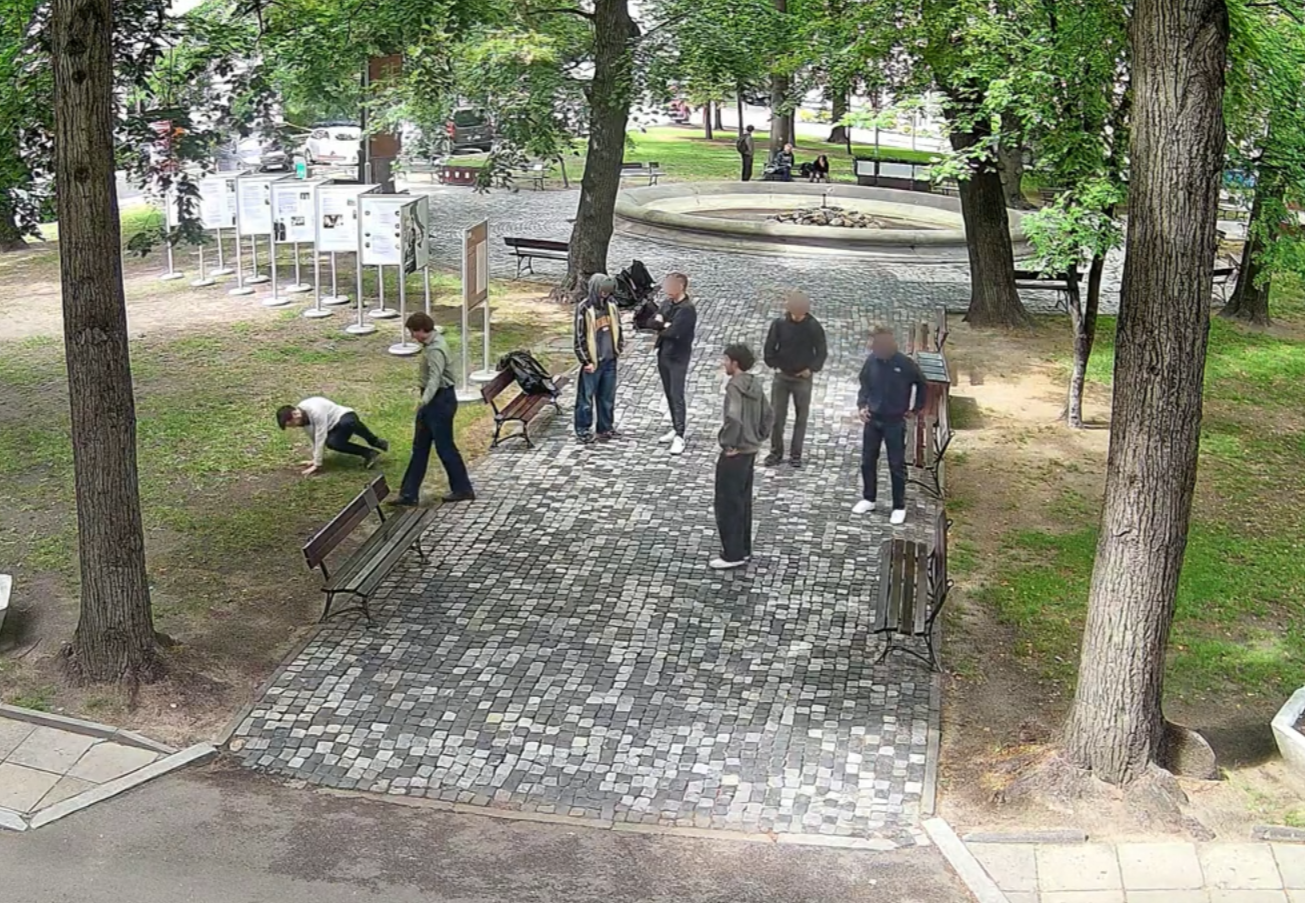
\includegraphics[width=0.95\textwidth]{images/detektor/upadek.png}
        \subcaption{Wykrycie upadku.}
    \end{subfigure}
    \hfill
    \begin{subfigure}{0.49\textwidth}
        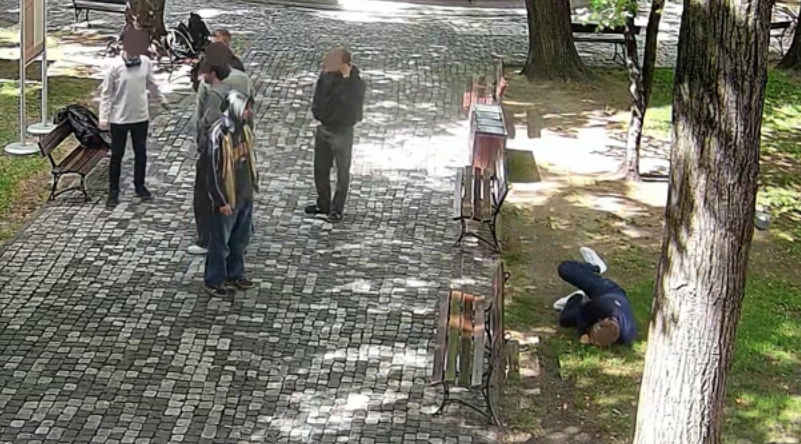
\includegraphics[width=0.95\textwidth]{images/detektor/upadek_2.png}
        \subcaption{Wykrycie upadku w innej scenie.}
    \end{subfigure}
    \caption{Przykłady poprawnej detekcji upadku człowieka.}\label{fig:detektor_upadki}
\end{figure-}

Wysoką dokładność osiągnięto również w wykrywaniu naruszeń stref zakazanych. System poprawnie rozpoznaje zarówno pełne wejścia osób w obręb wyznaczonych obszarów, jak i sytuacje graniczne, gdy postać znajduje się dopiero na samej krawędzi strefy. Świadczy to o precyzji wyznaczania punktu styku z podłożem względem zdefiniowanego wielokąta.

\begin{figure-}
    \centering
    \begin{subfigure}{0.49\textwidth}
        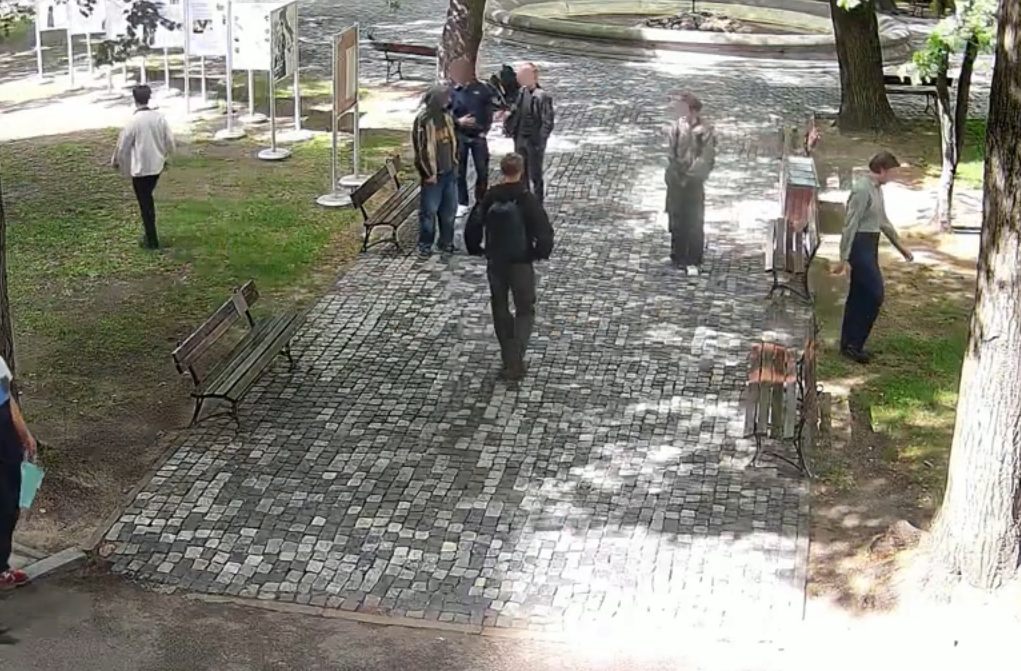
\includegraphics[width=0.95\textwidth]{images/detektor/strefa_trawnik_obie_full.png}
        \subcaption{Pełne wejście na obie strefy (lewy i prawy trawnik).}
    \end{subfigure}
    \hfill
    \begin{subfigure}{0.49\textwidth}
        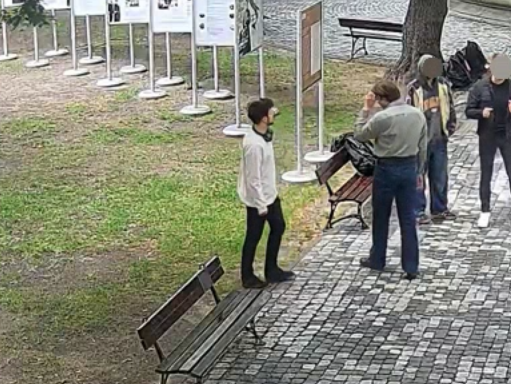
\includegraphics[width=0.95\textwidth]{images/detektor/strefa_trawnik_ledwo.png}
        \subcaption{Wejście na samą granicę strefy.}
    \end{subfigure}
    \caption{Detekcja naruszenia stref zakazanych: pełne wejście oraz sytuacja graniczna.}\label{fig:detektor_strefy}
\end{figure-}

Należy zaznaczyć ograniczenie wynikające z natury analizy opartej na ciągłości szkieletu. Przy chwilowym zasłonięciu osoby przebywającej w strefie, na przykład w wyniku przejścia za drzewem, detekcja może zostać przerwana: klasyfikator zachowań wymaga nieprzerwanego okna czasowego pozy, a wyznaczenie obecności w strefie zakłada widoczność punktu styku z podłożem. Gdy tylko postać ponownie staje się widoczna, detekcja jest wznawiana, dzięki czemu przerwy te są możliwie krótkie.

\subsection{Anonimizacja w praktyce}
Mechanizm anonimizacji skutecznie zabezpiecza dane wrażliwe. Twarze wielu osób jednocześnie, ustawionych pod różnymi kątami i z różnie zwróconymi głowami, zostają poprawnie zamazane. Jednocześnie osoba zwrócona tyłem do obiektywu, dla której model przypisuje oczom niskie prawdopodobieństwo, jest prawidłowo pomijana, co pozwala uniknąć zbędnych artefaktów.

\begin{figure-}
    \centering
    \begin{subfigure}{0.49\textwidth}
        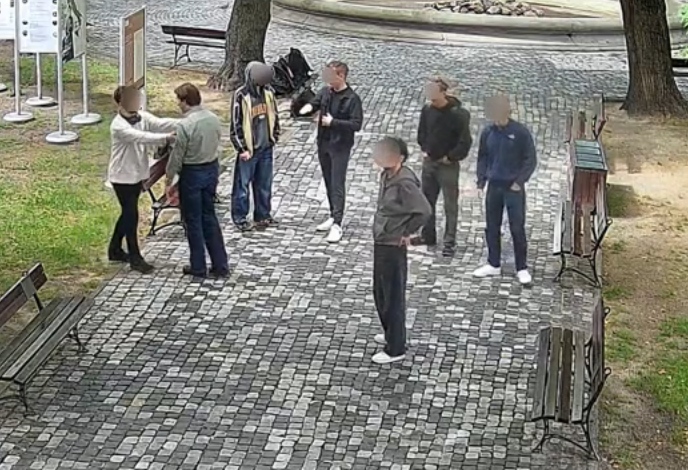
\includegraphics[width=0.95\textwidth]{images/detektor/rozmycie_twarzy.png}
        \subcaption{Rozmycie twarzy wielu osób.}
    \end{subfigure}
    \hfill
    \begin{subfigure}{0.49\textwidth}
        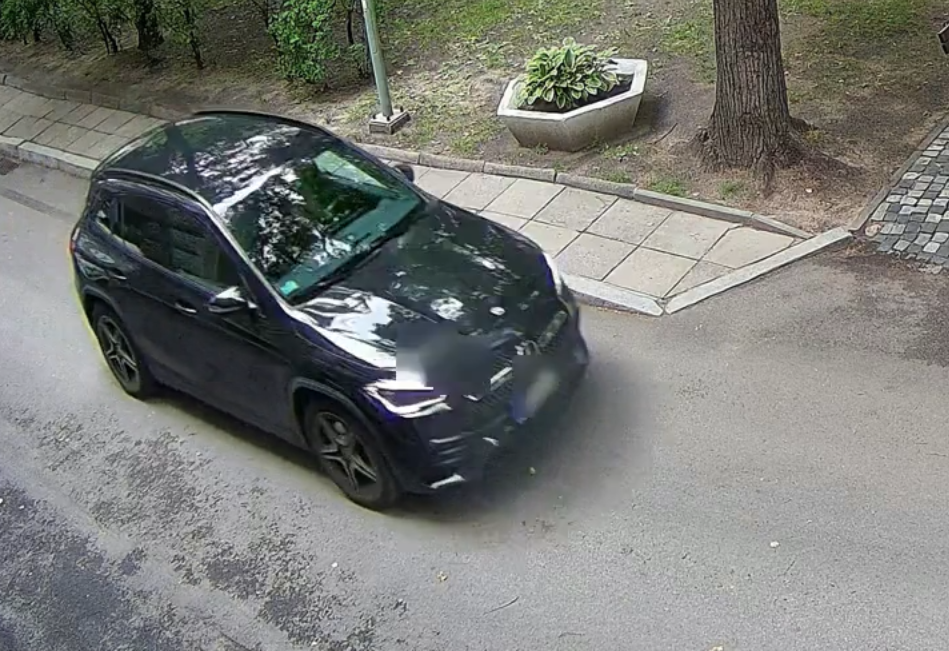
\includegraphics[width=0.95\textwidth]{images/detektor/auto.png}
        \subcaption{Rozmycie tablicy rejestracyjnej.}
    \end{subfigure}
    \caption{Działanie modułu anonimizacji: twarze przechodniów oraz tablica rejestracyjna pojazdu.}\label{fig:detektor_anonimizacja}
\end{figure-}

W przypadku tablic rejestracyjnych zdarza się, że maska rozmycia obejmuje również niewielki fragment nadwozia sąsiadujący z tablicą. Jest to nieznaczny efekt uboczny, który nie wpływa negatywnie na czytelność pozostałych cech pojazdu, a co najważniejsze, sama tablica pozostaje całkowicie nieczytelna, co jest zgodne z zamierzonym celem.

\subsection{Wpływ rozdzielczości przetwarzania}\label{subsec:detektor_imgsz}
Istotny wpływ na jakość detekcji ma stała \texttt{POSE\_IMGSZ} w module detektora, odpowiadająca parametrowi \texttt{imgsz} przekazywanemu do modeli YOLO, czyli rozmiarowi obrazu, do którego skalowana jest klatka przed inferencją. Im większa wartość tego parametru, tym dokładniejsza detekcja, szczególnie obiektów małych lub odległych od kamery (jak omawiana wcześniej klasa \texttt{knife}), lecz tym dłuższy czas przetwarzania pojedynczej klatki. Dobór tej wartości stanowi więc kompromis zależny od dostępnego sprzętu oraz od rozdzielczości obrazu wejściowego.

Przedstawione w podrozdziale~\ref{sec:detektor_wyniki} wyniki czasowe uzyskano przy wartości \texttt{POSE\_IMGSZ} równej 1600 na komputerze klasy domowej, co dało zadowalające opóźnienia przy zachowaniu wysokiej dokładności. Uruchomienie systemu na wydajniejszym sprzęcie pozwala podnieść ten parametr (a tym samym dokładność) bez pogorszenia bieżącości przetwarzania albo osiągnąć jeszcze krótsze opóźnienia przy zachowaniu dotychczasowej dokładności.


\chapter{System zarządzania wykrywanymi zachowaniami}
System zarządzania wykrywanymi zachowaniami stanowi główny element 
zarządzający danymi w projekcie. Komponent ten został zaimplementowany w języku \texttt{Java} z 
wykorzystaniem szkieletu aplikacji \texttt{Spring Boot}, co pozwoliło na uzyskanie wydajnego przetwarzania, 
skalowalności oraz modułowej architektury.

Głównym przeznaczeniem serwisu jest rola centralnego punktu integracyjnego całego systemu. 
Podsystem ten pośredniczy w komunikacji z modułami detekcji obrazu na żywo, 
przyjmując i weryfikując poprawność rejestrowanych incydentów, jak również udostępnia 
punkty końcowe wykorzystywane przez interfejs użytkownika. Serwis odpowiada za 
zarządzanie przechowywanymi danymi detekcji oraz udostępniania materiały wideo pełnych 
sekwencji detekcji do odczytu dla operatorów.

\section{Architektura modułu}

\subsection{Model składowania danych}
W celu zagwarantowania optymalnej wydajności i uniknięcia opóźnień podczas 
zapisu dużych plików, w infrastrukturze projektowej zaimplementowano hybrydowy model 
składowania danych. Do składowania różnych rodzajów danych zostały wykorzystane:
\begin{itemize}
    \item \textbf{Relacyjna baza danych (\texttt{PostgreSQL})} --- Odpowiada za składowanie ustrukturyzowanych danych mapowań przechowywanych nagrań oraz szablonów detekcji. W bazie danych przechowywane są również przekazywane przy zapisie nagrań wykrytych w nich elementów, z odpowiednimi znacznikami czasowymi.
    \item \textbf{Lokalny system plików (Pamięć dyskowa)} --- Stanowi fizyczny magazyn dla zapisywanych nagrań. Dane na dysku kategoryzowane wewnątrz struktury katalogów, których nazwy odpowiadają dacie rejestracji, a poszczególne pliki wideo posiadają w nazwie precyzyjny znacznik czasu ich zapisu, co umożliwia administratorom i operatorom, ich ręczną lokalizację bezpośrednio z poziomu systemu operacyjnego, gdyby zaszła taka potrzeba.
\end{itemize}

\begin{figure}[H]
    \centering

    \begin{subfigure}{\textwidth}
        \centering
        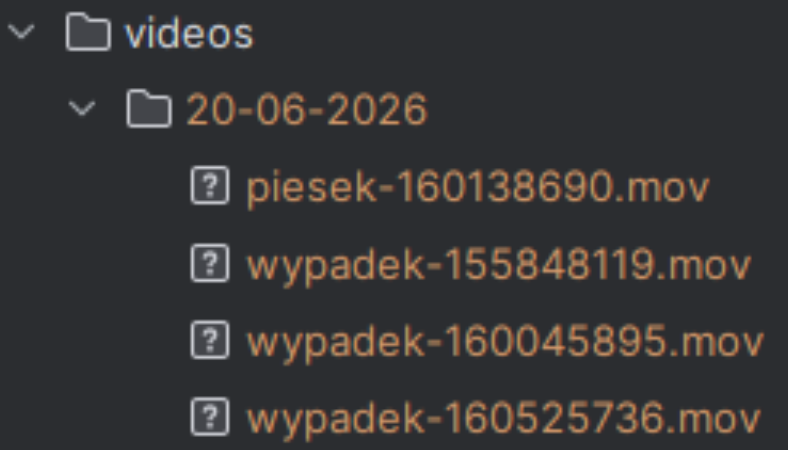
\includegraphics[width=0.4\linewidth]{images/przykladowy_stan_dysku_po_zapisie.png}
        \caption{Stan dysku z zapisanymi plikami nagrań detekcji.}
    \end{subfigure}

    \vspace{0.5cm}

    \begin{subfigure}{\textwidth}
        \centering
        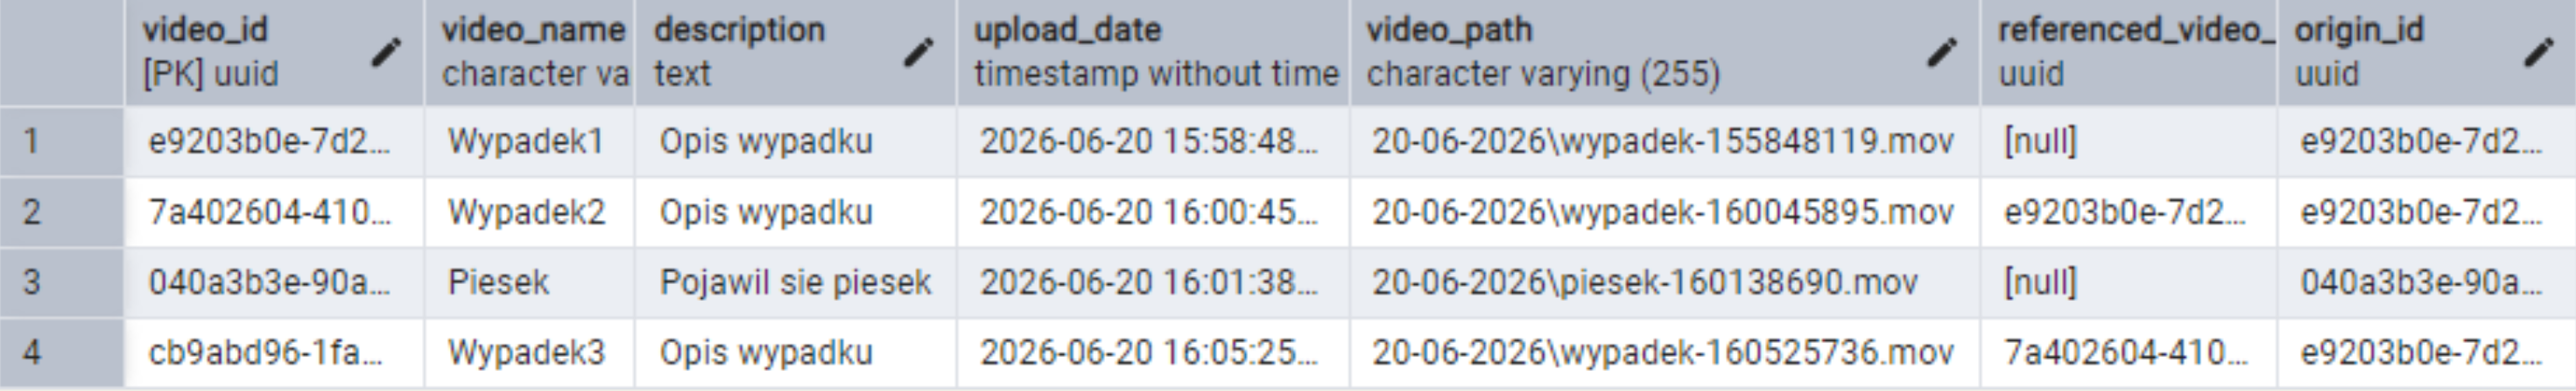
\includegraphics[width=0.95\linewidth]{images/przykladowy_stan_mapowan_w_bazie.png}
        \caption{Stan bazy danych ze zmapowanymi nagraniami.}
    \end{subfigure}

    \caption{Przykładowy stan dysku po zapisie nagrań fragmentów detekcji wraz z odzwierciedlającymi je mapowaniami zapisanymi w bazie danych.}
\end{figure}


\subsection{Architektura potoku zapisu i mapowania danych}
System zarządzania wykrywanymi zachowaniami w ramach zapisu i odczytu działa według zdefiniowanego potoku. 
Po wyemitowaniu przez detektor zestawu danych detekcji (pliku wideo wraz z opisem jego detekcji w formacie \texttt{JSON}), 
uruchamiana jest weryfikacja danych wejściowych. W ramach tej weryfikacji najpierw sprawdzana 
jest poprawność formatu pliku multimedialnego, co zapobiega próbom przesłania plików uszkodzonych 
lub obrazów statycznych zamiast strumienia wideo. Następnie system sprawdza poprawność składniową 
i budowę powiązanego dokumentu \texttt{JSON} zawierającego szczegóły detekcji.

Gdy walidacja zakończy się sukcesem, plik wideo jest fizycznie zapisywany w odpowiednim 
katalogu na dysku twardym. Po otrzymaniu systemowego potwierdzenia o prawidłowym zapisie pliku 
serwis zapisuje w bazie danych wiersz mapujący zapisany plik wideo w bazie \texttt{PostgreSQL}.
Rekord ten zawiera unikalne ID, ścieżkę dyskową oraz dwa kluczowe wskaźniki: 
\texttt{referenced\_video\_id} (ID filmu poprzedzającego w sekwencji) oraz 
\texttt{origin\_id} (ID elementu rozpoczynająca daną sekwencję wideo), co kończy proces zapisu.

Dopełnieniem potoku jest serwis synchronizujący, którego celem jest utrzymanie bezwzględnej 
spójności mapowań pomiędzy warstwą bazodanową a fizyczną zawartością dysku lokalnego. 
Ponieważ potok zapisu działa wieloetapowo, jakiekolwiek zakłócenia zewnętrzne 
(np.\ ręczne usunięcie pliku przez administratora lub awaria zasilania w trakcie trwania procedury) 
mogłyby doprowadzić do powstania mapowań wskazujących na nieistniejące zasoby. 
Z tego powodu serwis synchronizujący stale monitoruje efekty potoku zapisu, reagując natychmiastowo 
na zmiany w stanie plików, również w trakcie pracy systemu, Informując o dokonanych operacjach związanych
z synchronizacją. Zapewnia to, że przechowywane w bazie wiersze mapujące nagrania 
są zawsze bezwzględnym odzwierciedleniem stanu faktycznego zapisanych na dysku nagrań.

\begin{figure}[H]
    \centering
    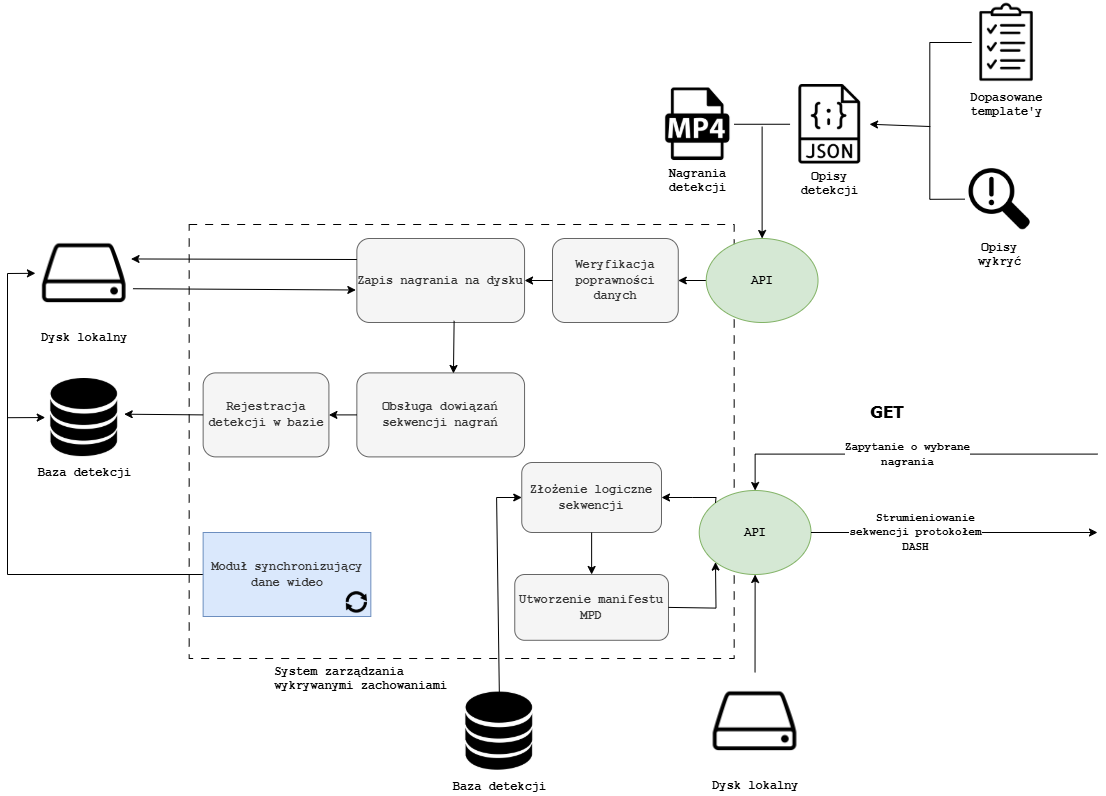
\includegraphics[width=0.9\textwidth]{images/diagram_backed.png}
    \caption{Architektura potoku zapisywania oraz odczytu i strumieniowania nagrań wideo.}
\end{figure}


\section{Opis funkcjonalności}

\subsection{Logika sekwencjonowania nagrań wideo}
Kluczową, w kontekście zapisywania nagrań z kamer, funkcjonalnością systemu jest możliwość 
rejestrowania długotrwałych zdarzeń bez przeciążania infrastruktury sieciowej. 
Funkcja ta realizowana jest poprzez mechanizm sekwencji, czyli logicznych list powiązanych, następujących
po sobie fragmentów wideo. Zamiast oczekiwać na zakończenie całego (możliwie kilkuminutowego) 
zdarzenia i wysyłać jeden duży plik, moduł detekcji sukcesywnie przesyła parosekundowe fragmenty detekcji. 
Zapewnia to informowanie operatorów o zagrożeniach w czasie rzeczywistym, co jest bardzo ważnym elementem, 
jeżeli system miałby zostać zastosowany w kontroli bezpieczeństwa.

Logika powiązań między nagraniami opiera się na strukturze listy jednokierunkowej 
generowanej w ramach zapisywanych mapowań do bazy danych. Jako ważne elementy sekwencji należy wymienić:
\begin{itemize}
    \item \textbf{origin} --- Pierwszy fragment rejestrujący początek incydentu. Wszystkie fragmenty należące do tego samego zdarzenia współdzielą ten sam \texttt{origin\_id}.
    \item \textbf{referenced\_video\_id} --- Każdy kolejny fragment przechowuje identyfikator swojego bezpośredniego poprzednika. Ten element bezpośrednio odpowiada za strukturę listy jednokierunkowej.
    %\item 
\end{itemize}
Zastosowanie wspólnego \texttt{origin\_id} eliminuje konieczność iteracyjnego, kosztownego przeszukiwania bazy „element po elemencie” podczas odczytu, kierując się jedynie dowiązaniami z \texttt{referenced\_video\_id}, przy wyszukiwaniu sekwencji. Zamiast tego system jednym zapytaniem \texttt{SQL} pobiera wszystkie rekordy o danym \texttt{origin\_id}, a dopiero następnie w pamięci \texttt{RAM} układane są one w prawidłowej kolejności przy wykorzystaniu \texttt{referenced\_video\_id}, przygotowując do wyświetlenia.

\begin{figure}[H]
    \centering
    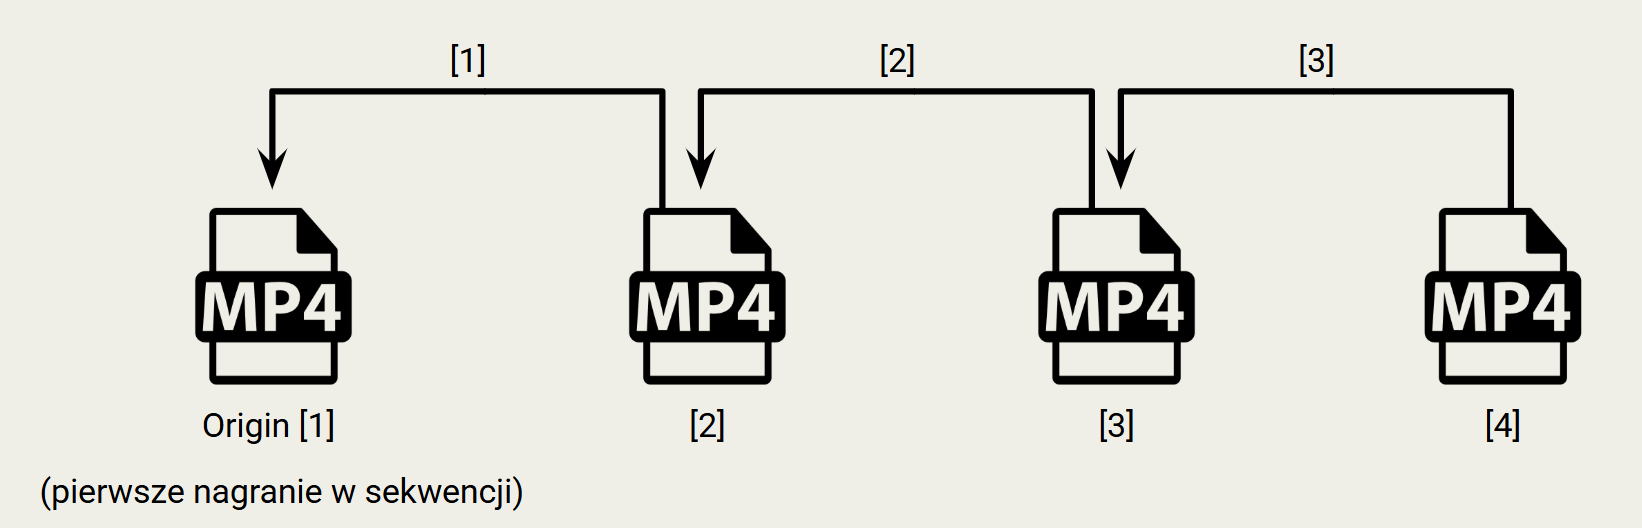
\includegraphics[width=0.8\textwidth]{images/przykladowa_sekwencja.png}
    \caption{Diagram logiczny struktury przykładowej sekwencji nagrań wideo.}
\end{figure}

\subsection{Mechanizm naprawy powiązań sekwencji}
System, poza usuwaniem całych sekwencji, pozwala z poziomu \texttt{API} na kasowanie pojedynczych, 
wybranych fragmentów z sekwencji danego zdarzenia. Rodzi to jednak ryzyko przerwania spójności 
referencyjnej i możliwości „osierocenia” pozostałych elementów sekwencji, co uniemożliwiłoby 
poprawne odtwarzanie filmu detekcji. W tym celu zaimplementowano mechanizm naprawy powiązań między 
elementami sekwencji. W jego ramach realizowane są trzy scenariusze:
\begin{enumerate}
    \item \textbf{Usunięty został element końcowy} --- Nie wymaga ingerencji, struktura listy pozostaje nienaruszona.
    \item \textbf{Usunięty został element środkowy} --- Algorytm modyfikuje mapowania fragmentów detekcji w bazie danych tak, aby element następujący po usuniętym wskazywał jako swój \texttt{referenced\_video\_id} na element stojący przed usuniętym fragmentem (przepięcie wskaźnika).
    \item \textbf{Usunięty został element inicjujący (origin)} --- Drugi w kolejności fragment w sekwencji zostaje pozbawiony wskaźnika \texttt{referenced\_video\_id} (staje się nowym początkiem, origin). We wszystkich elementach tej sekwencji wartość \texttt{origin\_id} zostaje nadpisana identyfikatorem nowego elementu początkowego.
\end{enumerate}

\subsection{Serwis synchronizujący mapowania danych}
Nad spójnością danych mapowań nagrań w bazie danych czuwa serwis synchronizujący. 
Zapobiega on powstawaniu martwych rekordów w bazie, gdy baza wskazuje na plik usunięty z poziomu dysku przez administratora. 
Usługa ta reaguje w trzech sytuacjach:
\begin{itemize}
    \item \textbf{Pomyślna weryfikacja startowa} --- Podczas uruchamiania serwisu system sprawdza zgodność mapowań w bazie z dyskiem. W przypadku pełnej spójności wysyłany jest komunikat potwierdzający integralność danych.
    \item \textbf{Synchronizacja przy rozruchu} --- Jeśli pliki zostały skasowane z dysku w czasie, gdy serwer był wyłączony, przy starcie system zidentyfikuje te braki i usuwa nieaktualne wpisy z bazy danych. Na koniec wyświetlany jest raport statystyczny informujący o liczbie usuniętych w ten sposób mapowań.
    \item \textbf{Synchronizacja w trakcie pracy systemu} --- Wszystkie modyfikacje plików na dysku podczas działania aplikacji są przechwytywane, a powiązane mapowania fragmentów nagrań w bazie, są również natychmiast usuwane.
\end{itemize}

\subsection{Zarządzanie szablonami detekcji}
Podsystem udostępnia pełną funkcjonalność zarządzania szablonami reguł za pośrednictwem \texttt{API} 
i powiązanego interfejsu webowego operatora. Użytkownik ma możliwość tworzenia, edycji, pobierania 
oraz usuwania konfiguracji szablonów. Każdy szablon ma unikalną nazwę oraz tablicę 
tzw.\ wektorów detekcji. Wektory definiują kombinacje oraz progi liczbowe obiektów 
(np.\ obecność minimum dwóch ludzi i jednego niebezpiecznego narzędzia). 
System udostępnia także dynamiczną listę aktualnie obsługiwanych klas obiektów, co pozwala 
interfejsowi webowemu na walidację wprowadzanych przez użytkownika definicji i zapobieganiu 
zapisywaniu błędnych reguł.

\subsection{Rejestracja i zapis nagrań detekcji}
Zapis fragmentów wideo oraz powiązanych z nimi opisów wykrytych elementów, otrzymanych 
bezpośrednio z modułu detektora, odbywa się za pośrednictwem punktu końcowego \texttt{REST API}.\
Ze względu na konieczność jednoczesnego przesyłania binarnego pliku multimedialnego (wideo) 
oraz ustrukturyzowanych danych tekstowych, żądanie to jest realizowane w formacie 
\texttt{multipart/form-data}. Format ten pozwala na niezależne przekazywanie różnych typów 
danych w ramach jednego zapytania \texttt{HTTP}.\

Po odebraniu tak sformułowanego żądania, system zarządzania wykrywanymi zachowaniami 
weryfikuje poprawność danych wejściowych, sprawdzając poprawność formatu pliku wideo, 
co zapobiega próbom przesłania plików uszkodzonych lub obrazów statycznych, 
a następnie waliduje budowę powiązanego dokumentu \texttt{JSON} zawierającego opis detekcji. 
Następnie plik wideo jest fizycznie zapisywany na dysku twardym w katalogu odpowiadającym dacie rejestracji, 
a do jego nazwy dopisywany jest precyzyjny znacznik czasowy. Dopiero po otrzymaniu potwierdzenia 
o prawidłowym zapisie pliku na dysku, serwis zapisuje w bazie \texttt{PostgreSQL} wiersz mapujący. 
Rekord ten wiąże fizyczny plik z unikalnym ID, ścieżką dostępu oraz wskaźnikami strukturalnymi 
sekwencji (\texttt{referenced\_video\_id} oraz \texttt{origin\_id}), co kończy proces zapisu.

W strukturze przesyłanego zapytania z modułu detekcji zawarte są następujące parametry wejściowe:
\begin{itemize}
    \item \texttt{file} --- Parametr zwierający surowe nagranie wideo z zarejestrowanym incydentem detekcji. Akceptowane są pliki w formacie \texttt{MP4} oraz \texttt{MOV}. Plik ten po przejściu walidacji formatu jest zapisywany w strukturze dyskowej serwera.
    \item \texttt{video-name}, \texttt{description} --- Określające nazwę oraz opis przypisane do danego fragmentu wideo. Wartości te nie są wykorzystywane w mapowaniu nagrania, a służą jedynie do wyświetlenia w interfejsie graficznym operatorowi.
    \item \texttt{relative-path} --- Ścieżka relatywna, która instruuje serwis, w jakim konkretnie miejscu wewnątrz katalogu nadrzędnego o określonej dacie ma zostać zapisany plik wideo na dysku lokalnym. Umożliwia to elastyczny zapis wideo mimo zastosowania automatycznie datowanych katalogów.
    \item \texttt{continuation-of} --- Opcjonalny parametr przechowujący identyfikator (ID) nagrania bezpośrednio poprzedzającego przesyłany fragment w strukturze sekwencji. Przekazanie tego parametru skutkuje automatycznym włączeniem nowego pliku do istniejącej już sekwencji wideo (jako kolejny element listy jednokierunkowej). W przypadku braku tego parametru system traktuje żądanie jako otwarcie zupełnie nowego incydentu i nadaje mu status elementu \textit{origin}.
    \item \texttt{details} --- Blok w formacie \texttt{JSON}, generowany moduł detektora. Zawiera on ustrukturyzowany opis detekcji, w tym wykaz klas wszystkich wykrytych obiektów oraz znaczniki czasowe określające zakres wykrycia elementów wewnątrz przesyłanego wideo.
\end{itemize}

\begin{figure}[H]
    \centering
    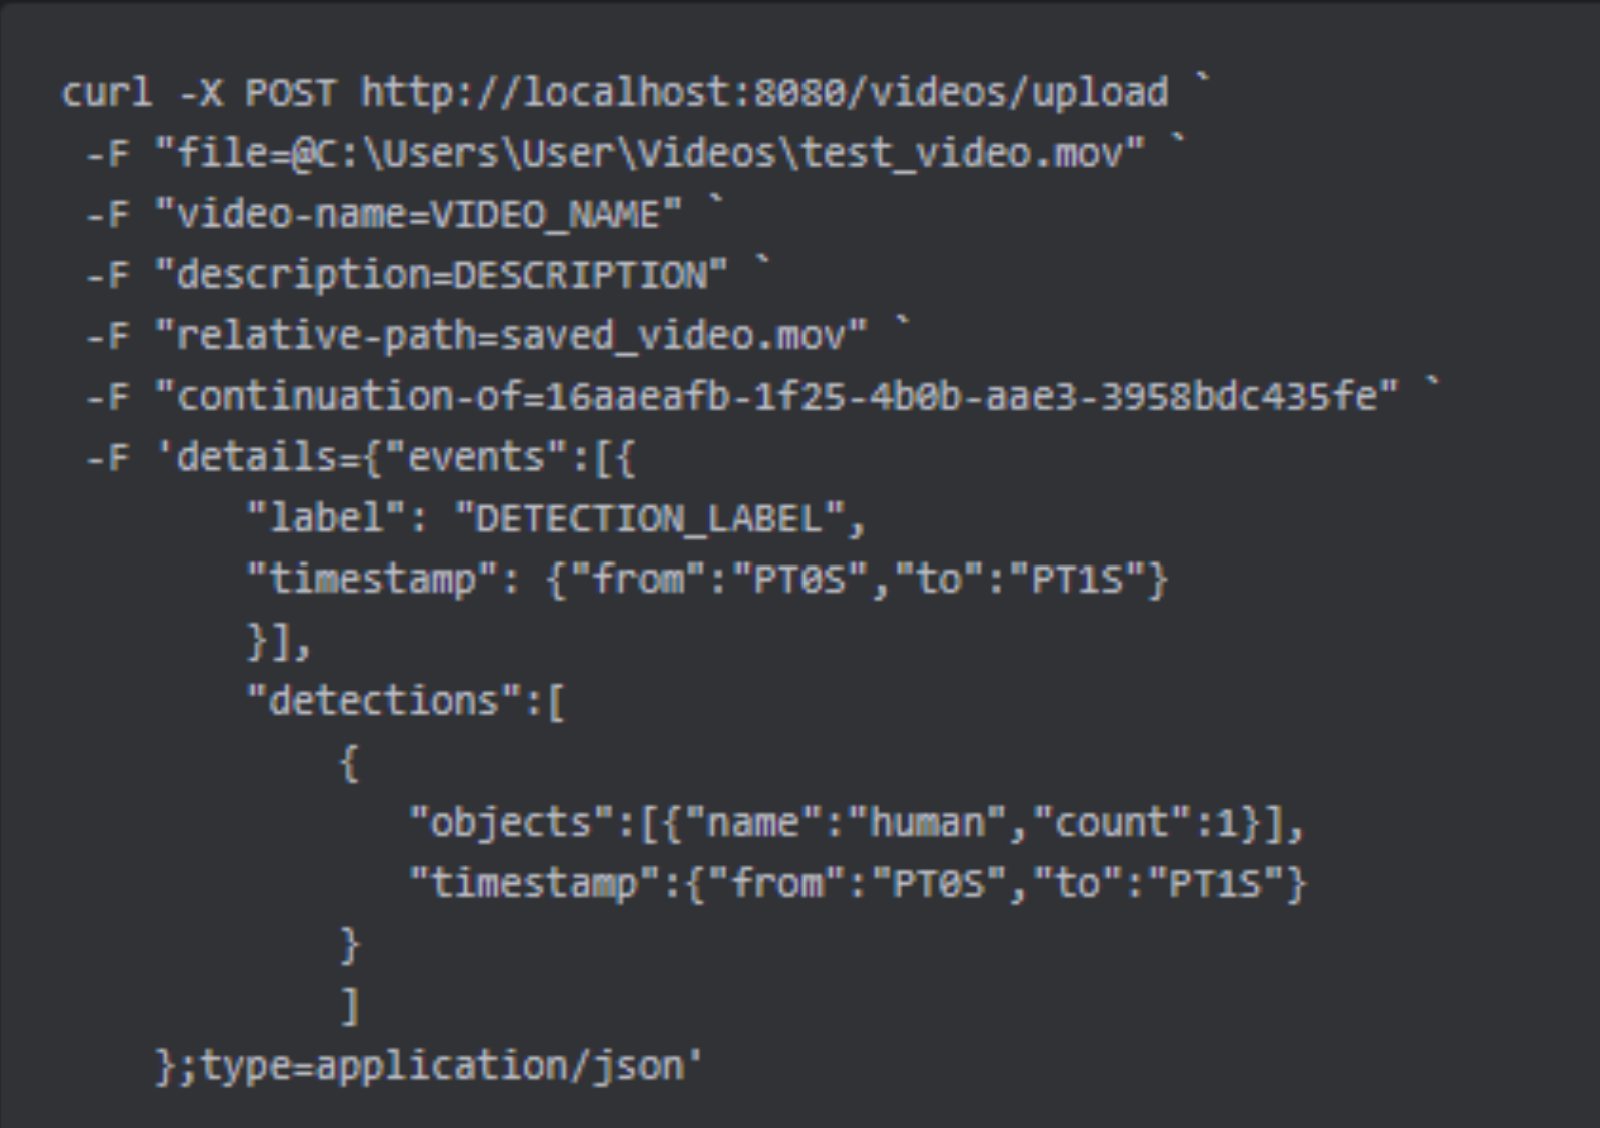
\includegraphics[width=0.8\textwidth]{images/przykladowe_zapytanie_zapisu_do_backendu.png}
    \caption{Przykładowe zapytanie zapisu detekcji.}
\end{figure}

\subsection{Strumieniowanie multimediów przy użyciu protokołu \texttt{DASH}}
Ostatnią kluczową funkcjonalnością jest dostarczanie wideo do interfejsu użytkownika obsługujące 
podzielone na fragmenty nagrania detekcji. System wykorzystuje do tego standard \texttt{DASH} 
(\textit{Dynamic Adaptive Streaming over HTTP}), opierając przesył danych o mechanizm częściowej 
zawartości (\textit{Partial Content}) przy wykorzystaniu kodu odpowiedzi \texttt{HTTP 206}. 

Na bazie logicznie ułożonej sekwencji, serwis generuje w locie manifest \texttt{XML} z rozszerzeniem 
\texttt{.mpd} (\textit{Media Presentation Description}). Dokument ten informuje odtwarzacz 
przeglądarki o osadzeniu czasowym poszczególnych fragmentów oraz adresach \texttt{URL}, 
pod którymi można je pobrać. Przeglądarka sekwencyjnie pobiera wyłącznie te fragmenty, 
które są niezbędne do zapełnienia bieżącego bufora odtwarzacza. 
Dla operatora korzystającego z interfejsu proces ten jest całkowicie niewidoczny. Pomimo 
fizycznego podzielenia danych na dysku, odtwarzany materiał zachowuje iluzję ciągłości nagrania,
przy jednoczesnym wyeliminowaniu opóźnień sieciowych i długiego buforowanie, jak w przypadku jednolitych
długich plików wideo.

\begin{figure}[H]
    \centering
    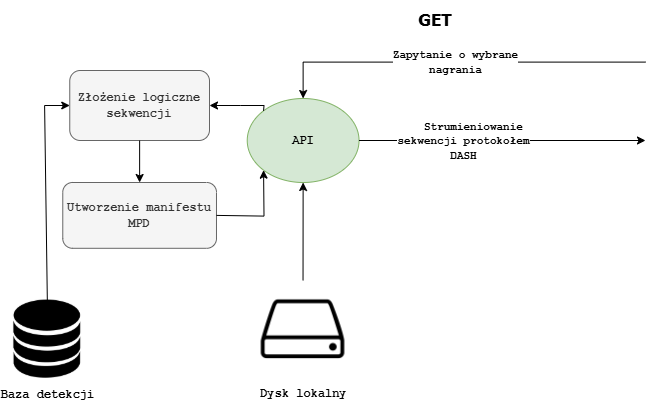
\includegraphics[width=0.7\textwidth]{images/Diagram_DASH.png}
    \caption{Potok odczytu sekwencji nagrań.}
\end{figure}
\chapter{Interfejs użytkownika}
Użytkownik wchodzi w interakcję z systemem poprzez aplikację webową, która jest dostępna w przeglądarce internetowej.
Za jej pomocą może on przeglądać strumienie wideo z kamer oraz zarządzać konfiguracją detekcji.

\section{Architektura modułu}
\subsection{Stos technologiczny}
Aplikacja webowa została zbudowana na podstawie szkieletu aplikacji \texttt{Next.js}. 
W roku 2026 najpopularniejszymi szkieletami aplikacji webowych pozostają \texttt{Vite} oraz właśnie \texttt{Next.js}.
Prawdopodobnie obie technologie sprawdziłyby się w tym projekcie, ale wybór padł na \texttt{Next.js} ze względu na to, że jest technologią nowszą.

Za warstwę wizualną odpowiada biblioteka \texttt{React}, która jest obecnie najpopularniejszą biblioteką do tworzenia interfejsów użytkownika w języku \texttt{JavaScript}. Zamiast klasycznego \texttt{JS} użyto jednak \texttt{TypeScript}, który wprowadza typowanie statyczne do języka \texttt{JavaScript}, co pozwala na wcześniejsze wykrywanie błędów w kodzie.

Warstwa stylistyczna została zrealizowana przy pomocy biblioteki \texttt{TailwindCSS}, która wprowadza gotowe klasy \texttt{CSS}, pozwalające na szybkie tworzenie estetycznych interfejsów użytkownika. Wykorzystano też gotowe komponenty z bilbioteki \texttt{shadcn/ui}, która jest zbiorem komponentów \texttt{React} stworzonych w oparciu o \texttt{TailwindCSS}. Część komponentów wzorowana jest na komponentach ze strony \href{https://flowbite.com}{\texttt{Flowbite}}.

Dodatkowo wykorzystano następujące biblioteki: 
\begin{itemize}
\item \texttt{Orval} --- biblioteka do generowania klienta API na podstawie specyfikacji \texttt{OpenAPI} (dawniej \texttt{Swagger}). Pozwala na automatyczne generowanie kodu, który umożliwia komunikację z serwerem poprzez protokół \texttt{HTTP}.
\item \texttt{Tanstack Query} --- biblioteka do zarządzania stanem aplikacji oraz komunikacją z serwerem. Umożliwia łatwe pobieranie danych z serwera oraz ich buforowanie w pamięci podręcznej, co pozwala na szybsze działanie aplikacji.
\item \texttt{Zustand} --- biblioteka do zarządzania stanem aplikacji. Umożliwia łatwe zarządzanie stanem globalnym w aplikacji \texttt{React}.
\item \texttt{Axios} --- biblioteka do wykonywania zapytań \texttt{HTTP}. Umożliwia łatwe wysyłanie zapytań do serwera oraz obsługę odpowiedzi.
\item \texttt{Shaka-Player} --- biblioteka do odtwarzania strumieni wideo w formacie \texttt{MPEG-DASH}. Umożliwia odtwarzanie strumieni wideo w przeglądarce internetowej.
\item \texttt{Zod} --- biblioteka do walidacji danych. Umożliwia łatwe sprawdzanie poprawności danych wprowadzanych przez użytkownika. 
\end{itemize}

\subsection{Implementacja}
\begin{figure}[H]
    \centering
    \begin{tikzpicture}[
        base/.style={draw, rectangle, rounded corners=3pt, align=center, font=\small, inner sep=5pt},
        external/.style={base, draw=red!60!black, fill=red!5!, thick, dashed, minimum width=5cm, minimum height=0.8cm},
        client/.style={base, draw=blue!60!black, fill=blue!5!, thick, minimum width=5cm, minimum height=0.8cm},
        comp/.style={base, draw=green!60!black, fill=green!5!, minimum width=2.4cm},
        hook/.style={base, draw=purple!70!black, fill=purple!5!, font=\scriptsize, minimum width=1.1cm},
        store/.style={base, draw=orange!70!black, fill=orange!5!, font=\scriptsize, minimum width=1.1cm},
        box/.style={draw=gray!40, fill=gray!5, dashed, rounded corners=5pt, inner sep=10pt},
        boxtitle/.style={font=\small\bfseries, text=gray!80!black},
        arrow/.style={-{Stealth[scale=1.2]}, thick, draw=gray!80!black},
        botharrow/.style={{Stealth[scale=1.2]}-{Stealth[scale=1.2]}, thick, draw=gray!80!black},
        dot/.style={circle, fill=gray!60, inner sep=0pt, minimum size=4pt}
    ]
    % 1. WARSTWA PODSTAWOWA (DÓŁ)
    \node[external] (api) {Zewnętrzny Serwer API\\(np. \texttt{FastAPI})};
    \node[client, above=1.2cm of api] (client) {Klient API (Axios / Fetch)};
    % 2. KOLUMNY FUNKCJONALNOŚCI (ŚRODEK I GÓRA)
    % --- FUNKCJONALNOŚĆ 1 (Lewa) ---
    \node[hook, above left=1.8cm and 1.2cm of client.north] (h1) {Hook};
    \node[store, right=0.2cm of h1] (s1) {Store};
    \node[comp, above=0.6cm of h1.north east] (c1) {Komponent UI};
    % --- FUNKCJONALNOŚĆ 2 (Prawa) ---
    \node[hook, above right=1.8cm and 1.2cm of client.north] (h2) {Hook};
    \node[store, right=0.2cm of h2] (s2) {Store};
    \node[comp, above=0.6cm of h2.north east] (c2) {Komponent UI};
    % 3. GENEROWANIE KONTENERÓW (TŁO)
    \begin{scope}[on background layer]
        \node[box, fit=(h1) (s1) (c1)] (box1) {};
        \node[box, fit=(h2) (s2) (c2)] (box2) {};
    \end{scope}
    % Podpisy pod kontenerami
    \node[boxtitle, above=2pt of box1.north] {Funkcjonalność 1};
    \node[boxtitle, above=2pt of box2.north] {Funkcjonalność 2};
    % --- TRZY KROPKI Z PRAWEJ STRONY ---
    \node[right=1.2cm of box2] (ellipsis) {};
    \node[dot, left=5pt of ellipsis] {};
    \node[dot] at (ellipsis) {};
    \node[dot, right=5pt of ellipsis] {};
    % 4. POŁĄCZENIA (STRZAŁKI)
    \draw[botharrow] (api) -- node[right, font=\tiny, text=gray!60!black] {HTTP / JSON} (client);
    \draw[arrow] (client.north) -- (box1.south);
    \draw[arrow] (client.north) -- (box2.south);
    \draw[arrow] (h1.north) -- (c1.south west);
    \draw[arrow] (s1.north) -- (c1.south east);
    \draw[arrow] (h2.north) -- (c2.south west);
    \draw[arrow] (s2.north) -- (c2.south east);
    \end{tikzpicture}
    \caption{Modularny podział warstwy prezentacyjnej z wyodrębnieniem domen funkcjonalnych.}\label{fig:modular_architecture_diagram}
\end{figure}
Aplikacja jest jednostronna (ang. \textit{Single Page Application}), co oznacza, że nie wykorzystuje ona trasowania po stronie serwera i działa jedynie w korzeniu domeny.

Zastosowana architektura modułu interfejsu użytkownika jest zorientowana na funkcjonalności (ang. \textit{Feature-Driven Architecture}). Oznacza to, że każda funkcjonalność ma własne komponenty interfejsu użytkownika, jak i również magazyny i hooki. Część podmodułów jest wspólna dla całego modułu, np.\ komponenty \texttt{shadcn/ui}. Podobnie jest z klientem API, z którego korzystają wszystkie funkcjonalności. 

Wspomniane hooki i magazyny (ang. \textit{store}) są wykorzystywane do zarządzania stanem aplikacji. Mają one jednak różne zastosowania. Magazyny przechowują te dane, które modyfikowane są przez użytkownika np.\ zaznaczone nagrania do usunięcia. Z kolei hooki są wykorzystywane do pobierania danych z serwera i ich buforowania w pamięci podręcznej. Dodatkowo częściowo realizują też komunikację w drugą stronę, np.\ przekazując nowe szablony detekcji. 

\section{Opis funkcjonalności}

\subsection{Obsługa motywów}
Moduł interfejsu użytkownika obsługuje dwa motywy: jasny i ciemny. Co prawda nie istnieje żaden przełącznik w interfejsie użytkownika, który pozwalałby na zmianę motywu, ale można to uczynić poprzez zmianę ustawień systemowych w przeglądarce internetowej, do której dopasowuje się aplikacja.

\begin{figure}[H]
    \centering
    \begin{subfigure}{0.45\textwidth}
        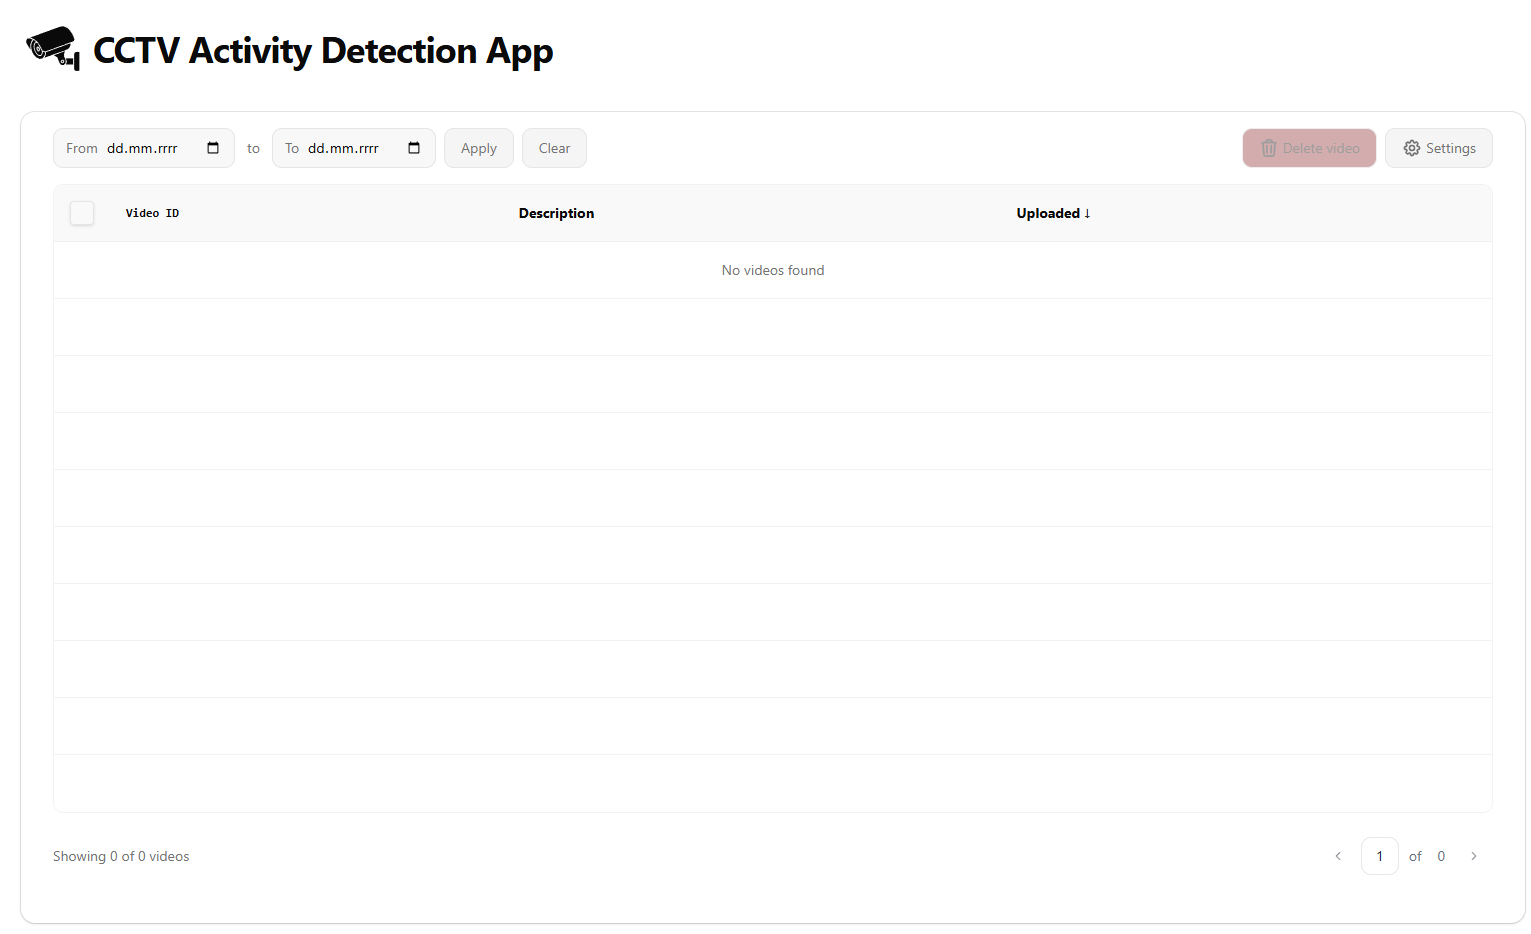
\includegraphics[width=0.95\textwidth]{images/frontend/interfejs_jasny.png}
        \subcaption{Motyw jasny.}\label{fig:frontend_light_theme}
    \end{subfigure}
    \hfill
    \begin{subfigure}{0.45\textwidth}
        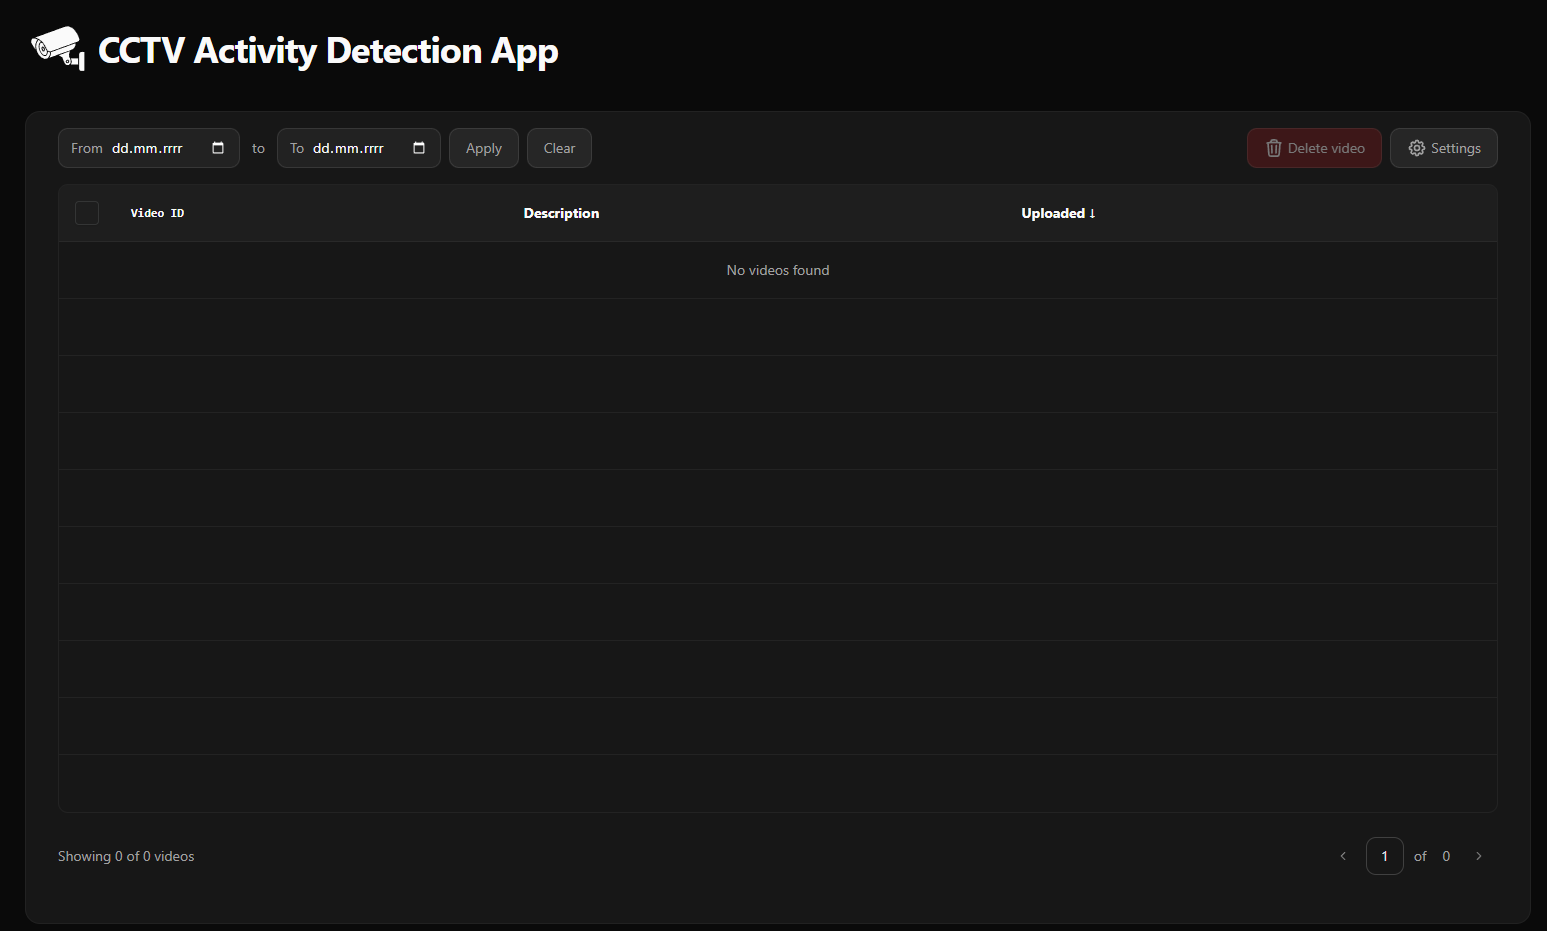
\includegraphics[width=0.95\textwidth]{images/frontend/interfejs_ciemny.png}
        \subcaption{Motyw ciemny.}\label{fig:frontend_dark_theme}
    \end{subfigure}

    \caption{Widok aplikacji w motywach jasnym i ciemnym.}
\end{figure}

\subsection{Lista i wyświetlacz nagrań}

\begin{figure}[H]
    \centering
    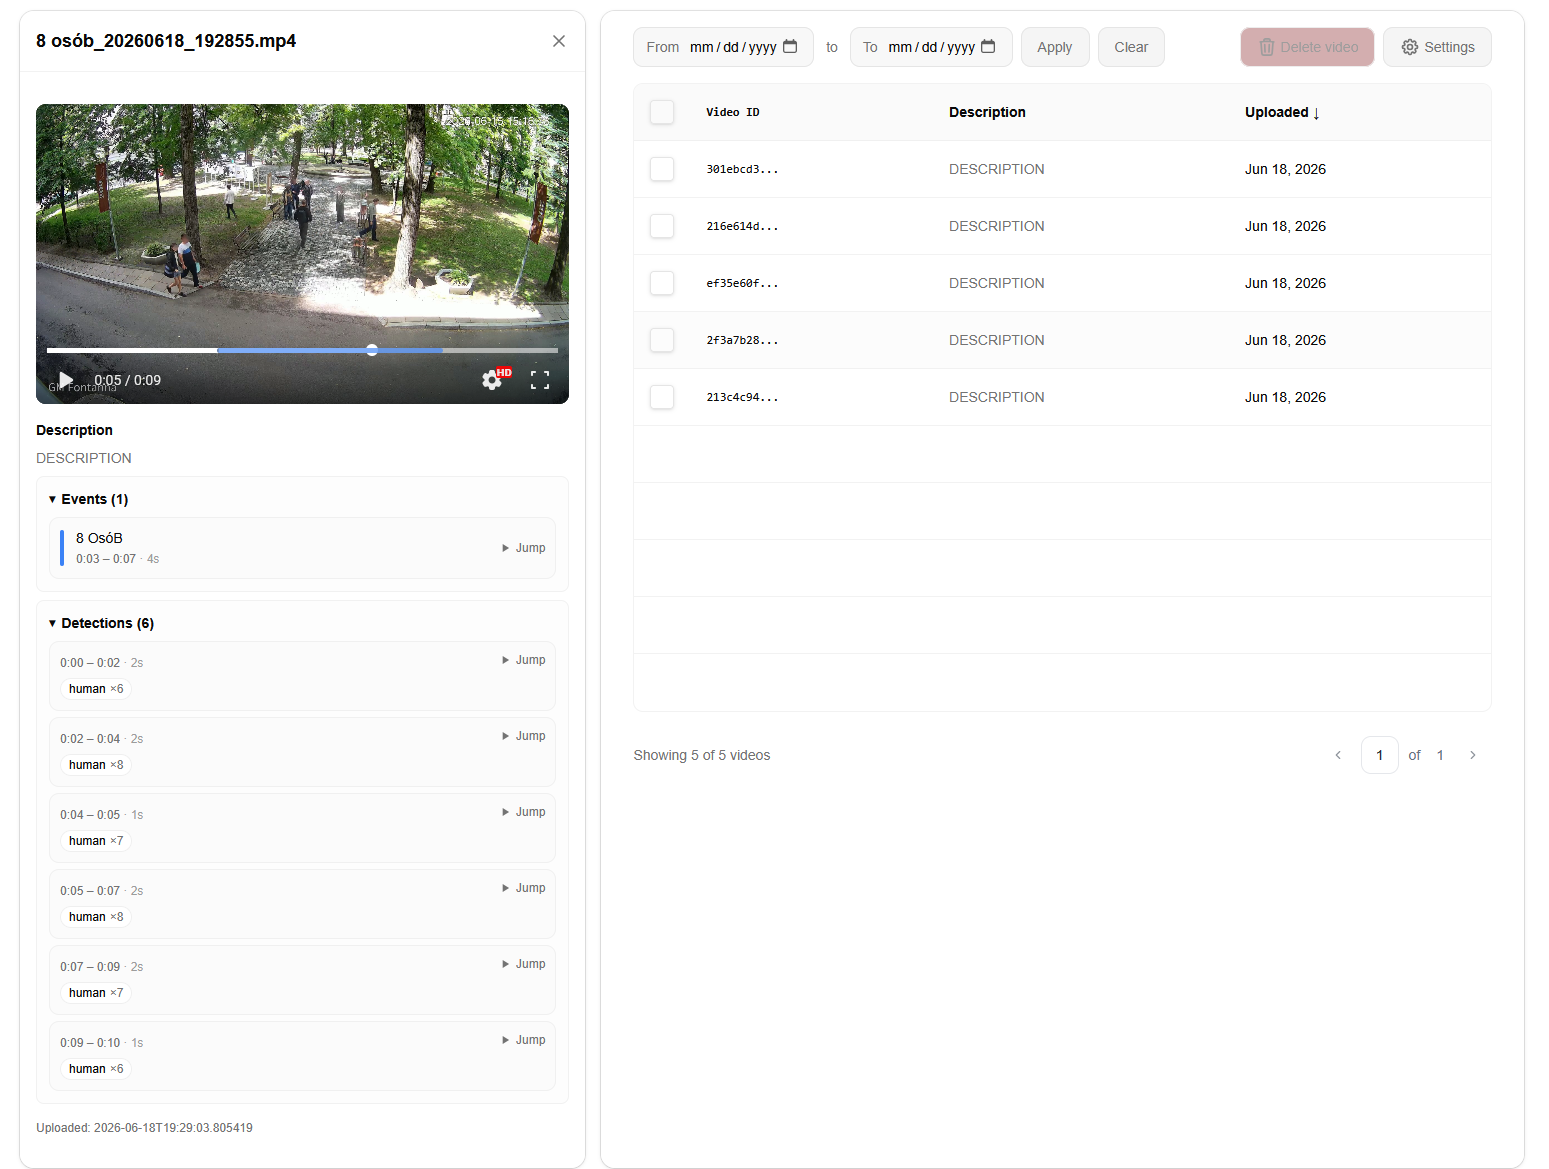
\includegraphics[width=0.95\textwidth]{images/frontend/interfejs.png}
    \caption{Lista nagrań wideo z możliwością ich odtwarzania.}\label{fig:frontend_recordings_list}
\end{figure}

Na \myref[rysunku]{fig:frontend_recordings_list} przedstawiono listę nagrań wideo. Widać, że jest ich pięć (\textit{Showing 5 of 5 videos}) oraz że wszystkie są na jednej stronie (\textit{1 of 1}). Każde nagranie posiada opis (nie zaimplementowano uzyskiwania opisów za pomocą wizyjnego modelu językowego), listę zarejestrowanych zdarzeń oraz zarejestrowanych detekcji z przedziałami czasowymi, w których mają miejsce.
Wyświetlacz nagrań można zmaksymalizować, ale wbrew temu, co może sugerować umieszczona na nim zębatka, niemożliwa jest zmiana jakości przesyłanego strumienia wideo. 

\subsubsection{Filtrowanie po dacie}
\begin{figure}[H]
    \centering
    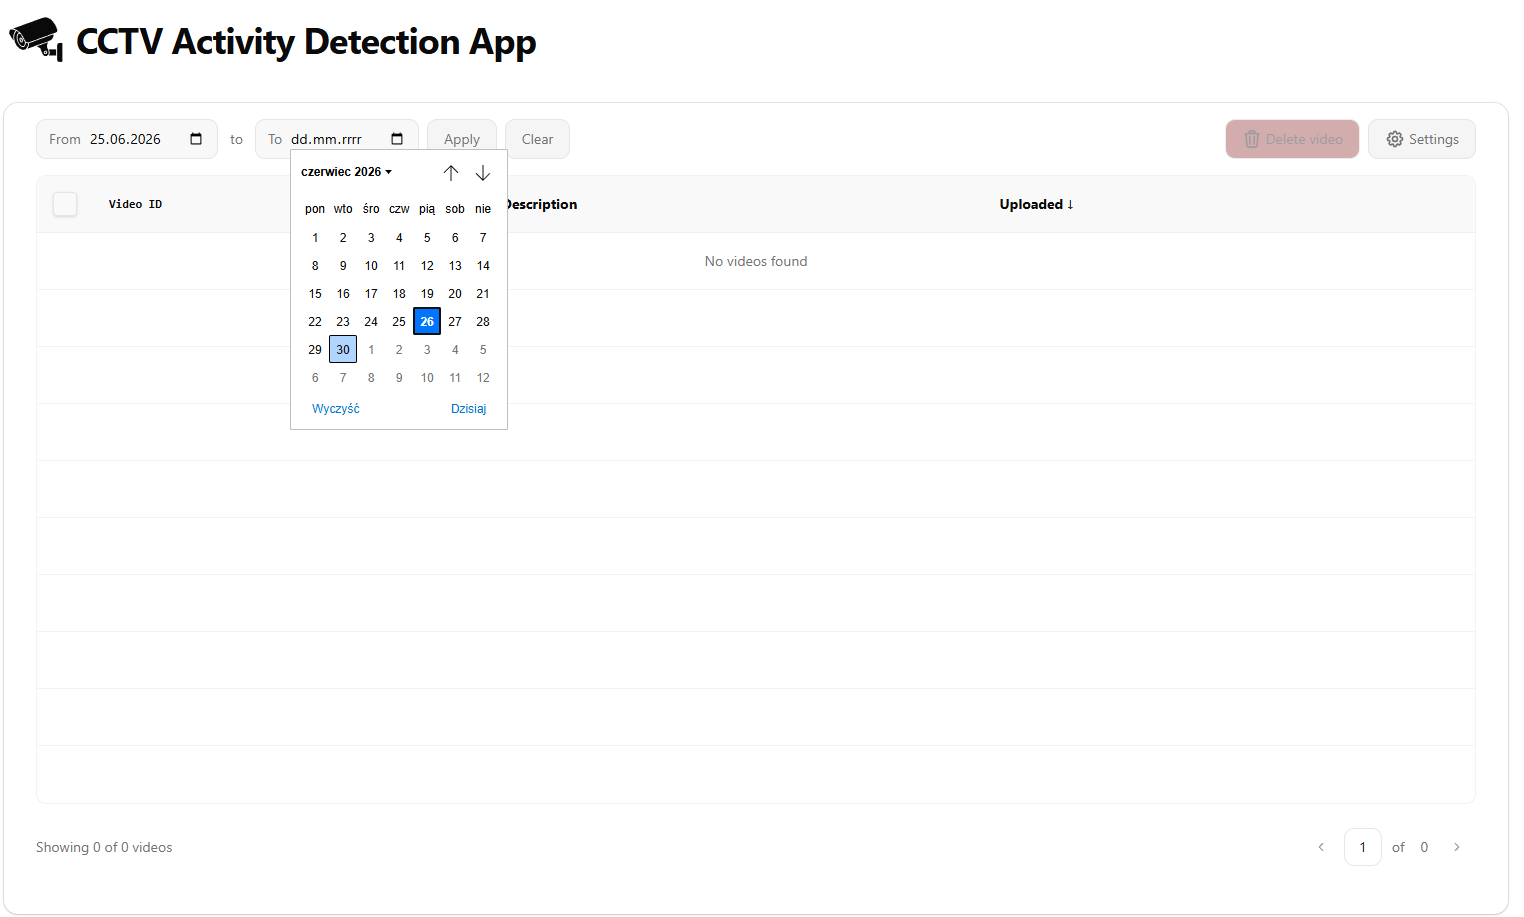
\includegraphics[width=0.95\textwidth]{images/frontend/filtrowanie.png}
    \caption{Filtrowanie nagrań wideo po dacie.}\label{fig:frontend_date_filter}
\end{figure}

Aplikacja umożliwia filtrowanie nagrań wideo po dacie. Na \myref[rysunku]{fig:frontend_date_filter} przedstawiono widok, na którym wybrano już dolny przedział daty od 25 czerwca 2026 r., a górny jest dopiero w trakcie wybierania. Nie wyświetliło się żadne z nagrań.

\subsubsection{Usuwanie nagrań}
\begin{figure}[H]
    \centering
    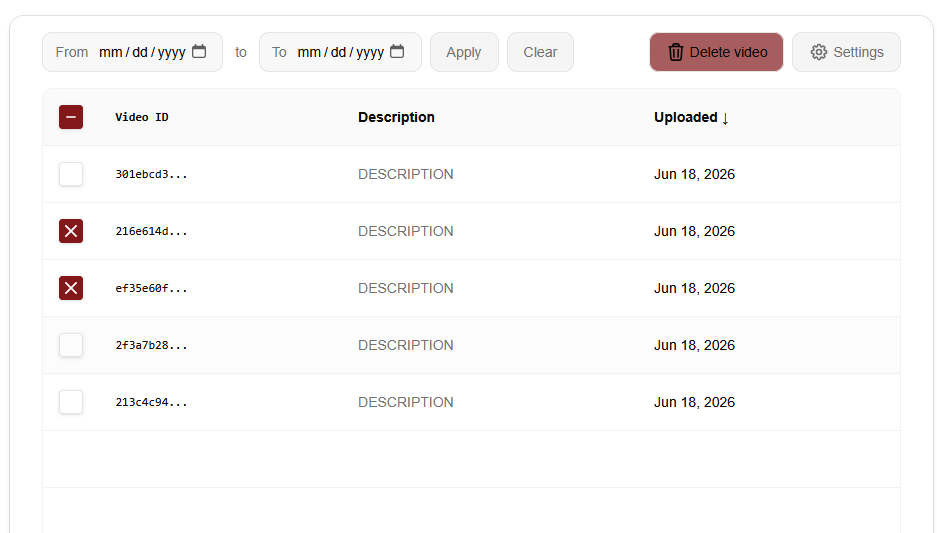
\includegraphics[width=0.95\textwidth]{images/frontend/usuwanie.png}
    \caption{Usuwanie nagrań wideo.}\label{fig:frontend_delete_recordings}
\end{figure}
Powyższy rysunek przedstawia zaznaczone do usunięcia nagrania wideo. Po kliknięciu przycisku \textit{Delete video} na serwer API trafi żądanie usunięcia nagrań z bazy danych.

\subsection{Ustawienia detekcji zdarzeń}

\begin{figure}[H]
    \centering
    \begin{subfigure}{0.49\textwidth}
        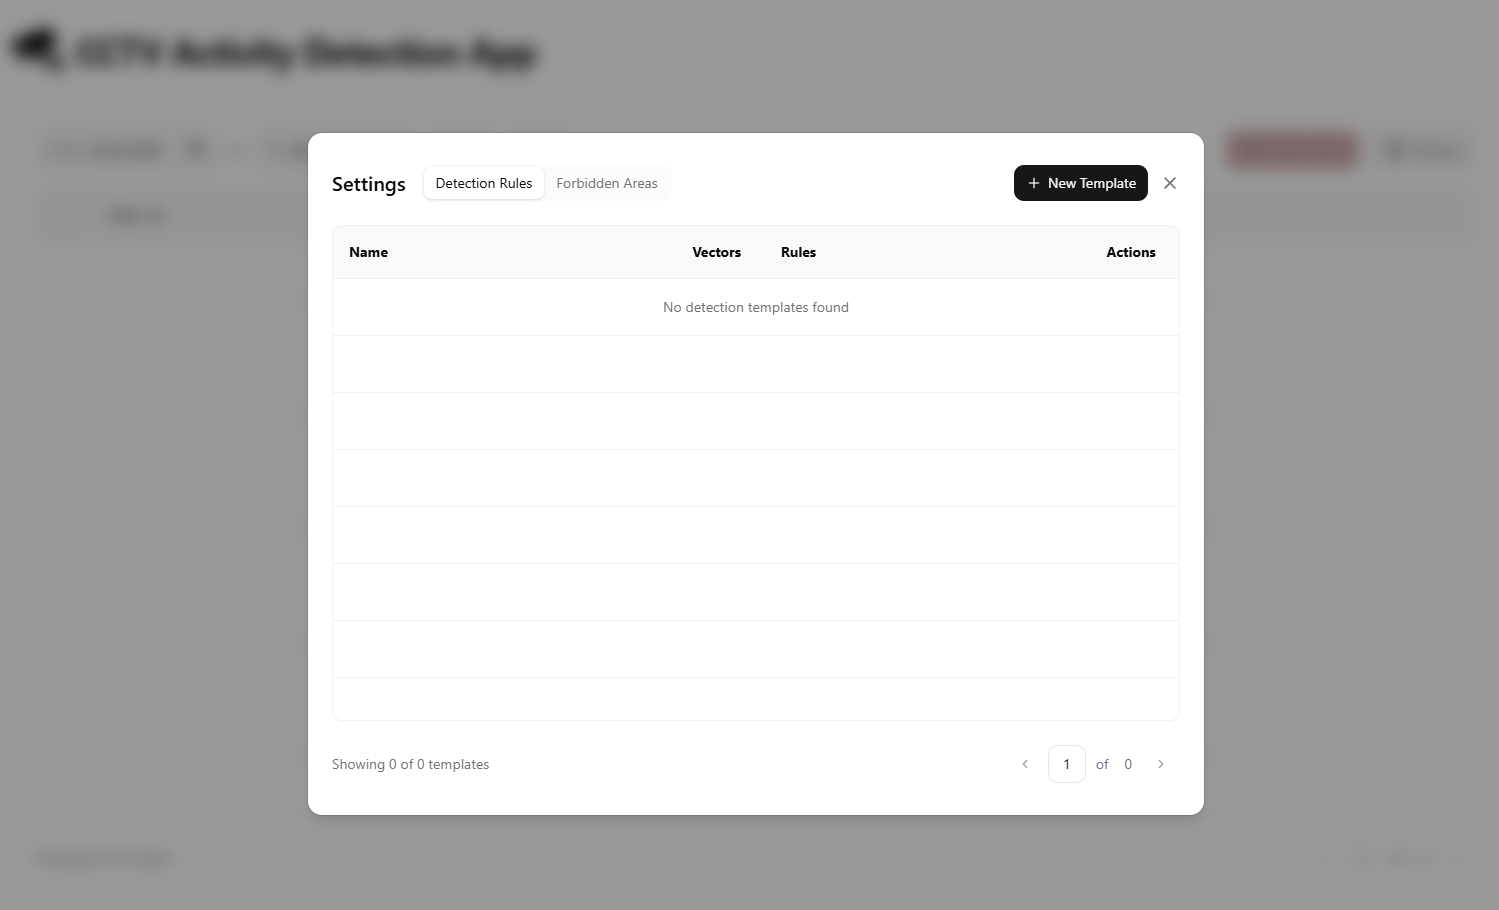
\includegraphics[width=0.95\textwidth]{images/frontend/zasady_wykrywania.png}
        \subcaption{Szablony detekcji.}
    \end{subfigure}
    \hfill
    \begin{subfigure}{0.49\textwidth}
        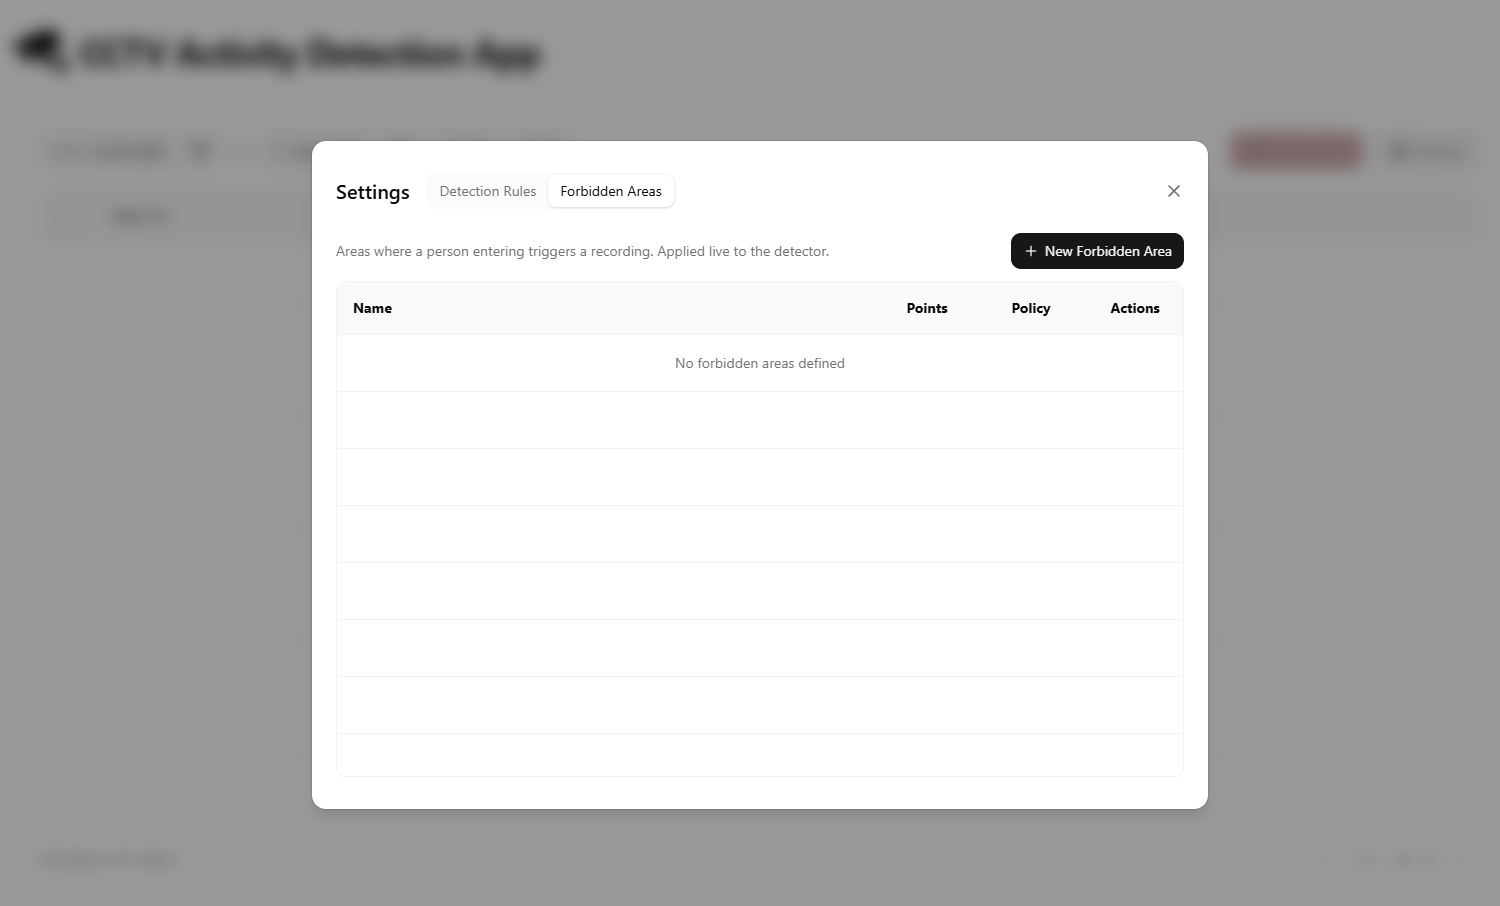
\includegraphics[width=0.95\textwidth]{images/frontend/zakazane_obszary.png}
        \subcaption{Wykrywane obszary.}
    \end{subfigure}
    \caption{Widok ustawień.}\label{fig:frontend_settings}
\end{figure}

Ustawienia dzielą się na dwie sekcje przedstawione na \myref[rysunku]{fig:frontend_settings}. W pierwszej z nich użytkownik może zarządzać szablonami detekcji, a w drugiej wykrywanymi obszarami.
\begin{figure}[H]
    \centering
    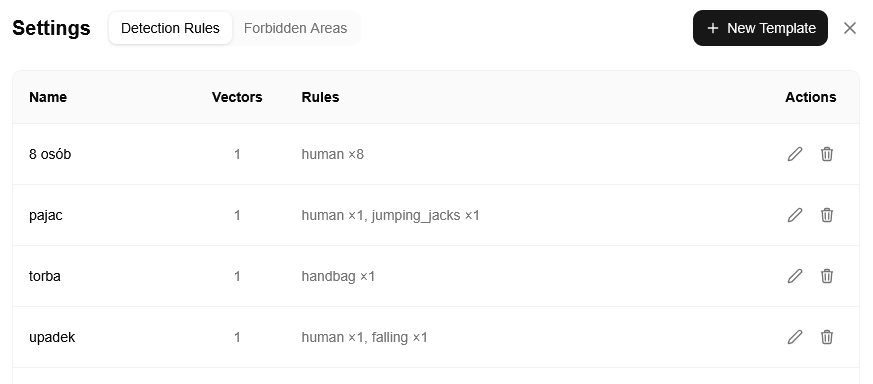
\includegraphics[width=0.95\textwidth]{images/frontend/wektory_wykryc.png}
    \caption{Przykład wprowadzonych szablonów wykryć.}\label{fig:frontend_detection_vectors}
\end{figure}

Jak widać na \myref[rysunku]{fig:frontend_detection_vectors}, użytkownik może zarządzać wprowadzonymi szablonami wykryć poprzez ich edycję, dodawanie i usuwanie.

\begin{figure}[H]
    \centering
    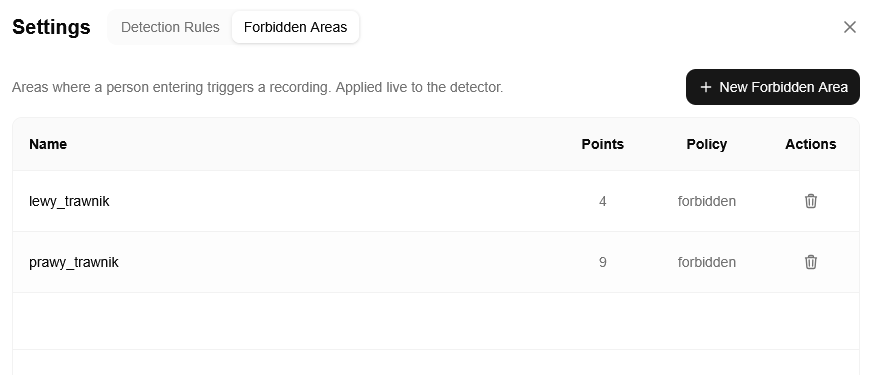
\includegraphics[width=0.95\textwidth]{images/frontend/obszary_wykluczone.png}
    \caption{Przykład wprowadzonych zakazanych obszarów.}\label{fig:frontend_restricted_areas}
\end{figure}

W przypadku zakazanych obszarów niemożliwe jest ich edytowanie, a jedynie dodawanie i usuwanie. Na \myref[rysunku]{fig:frontend_restricted_areas} pokazane są dwa zakazane obszary, które zostały wprowadzone przez użytkownika.

\subsection{Dodawanie szablonów detekcji}
\begin{figure}[H]
    \centering
    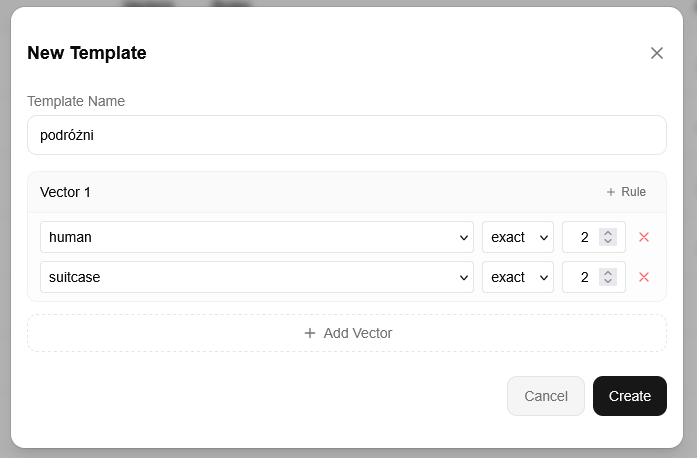
\includegraphics[width=0.95\textwidth]{images/frontend/wektor_podrozni.png}
    \caption{Przykład dodawania szablonu wykryć.}
\end{figure}
Powyższy rysunek przedstawia dodawanie szablonu wykryć. W tym przypadku użytkownik wprowadza szablon złożony z pojedynczego wektora, który wykrywa 2 ludzi i 2 teczki. Samo wprowadzenie szablonu nie wystarcza, aby zapisał się on w bazie danych. Konieczne jest wciśnięcie przycisku \enquote{Create}.

\subsection{Dodawanie zakazanych obszarów}
\begin{figure}[H]
    \centering
    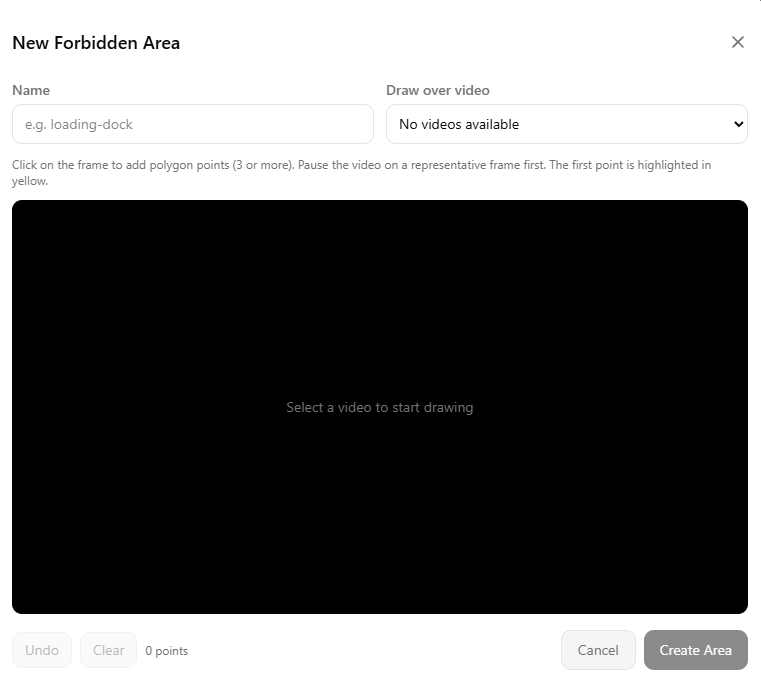
\includegraphics[width=0.95\textwidth]{images/frontend/zakazane_obszary_dodawanie.png}
    \caption{Przykład dodawania zakazanego obszaru.}
\end{figure}
Funkcjonalność pozwala na tworzenie wielokątów na obrazie z kamery, które będą traktowane jako zakazany obszar. Poniżej przykłady obszarów lewego i prawego trawnika:
\begin{figure}[H]
    \centering
    \begin{subfigure}{0.49\textwidth}
        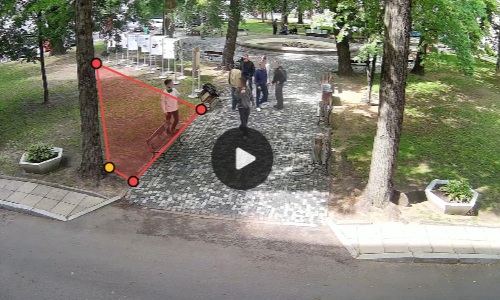
\includegraphics[width=0.95\textwidth]{images/frontend/lewy_trawnik.png}
        \subcaption{Lewy trawnik.}
    \end{subfigure}
    \hfill
    \begin{subfigure}{0.49\textwidth}
        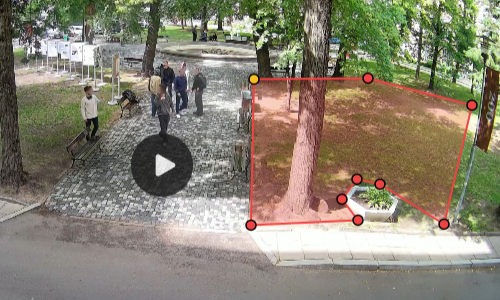
\includegraphics[width=0.95\textwidth]{images/frontend/prawy_trawnik.png}
        \subcaption{Prawy trawnik.}
    \end{subfigure}
    \caption{Zaznaczone obszary.}\label{fig:frontend_grass_areas}
\end{figure}
Wymagane jest zatem, aby w bazie danych były już zarejestrowane jakieś nagrania wideo, aby można było na ich podstawie wyznaczyć zakazane obszary. 

\include{chapters/wyniki}
\chapter{Podsumowanie}
Pomyślnie zrealizowano wszystkie założone cele projektu. Wytworzono moduły detektora, serwera API oraz serwera webowego.\ Detektor rozpoznaje zdarzenia na nagraniu testowym, prawidłowo anonimizuje twarze wykrytych osób.\ W trakcie prac zidentyfikowano problem związany z rozdzielczością obrazu. Moduł detektora wymagał precyzyjnego dopasowania hiperparametrów do specyfiki kamery testowej, aby zapewnić wysoką skuteczność wykrywania obiektów na rejestrowanych nagraniach.

\section{Dalsze możliwości rozwoju}
Istnieje wiele potencjalnych ścieżek rozwoju, jakie może przyjąć projekt. Możliwe jest m.in.:
\begin{enumerate}
\item Zwiększenie liczby wykrywanych obiektów i zdarzeń;
\item Zoptymalizowanie pętli przetwarzania klatek nagrań;
\item Dodanie mechanizmu uwierzytelniania i autoryzacji w interfejsie użytkownika;
\item Dodanie generowania dodatkowych opisów zdarzeń np.\ za pomocą modeli wizyjno-językowych;
\item Zabezpieczenie punktów końcowych serwera \texttt{API} przed nieupoważnionym dostępem;
\item Zastosowanie obecnego systemu w grze terenowej, w której gracze będą musieli wykonywać określone czynności na kamerach monitoringu. 
\end{enumerate}
Dzięki swojej modularnej budowie system może być rozbudowywany o nowe funkcjonalności, a obecny interfejs graficzny może zostać zastąpiony innym, gdyby zaszła taka potrzeba. Warto byłoby poważnie rozważyć
zabezpieczenie serwera \texttt{API} przed nieupoważnionym dostępem, aby zbierane nagrania z kamer były dodatkowo chronione. Można rozważyć czy gromadzone nagrania nie powinny być przechowywane w datalake'u, aby
zapewnić większą skalowalność i bezpieczeństwo danych. Możliwości rozwoju projektu są szerokie i nie brakuje pomysłów na jego dalszą rozbudowę.


\printbibliography
\end{document}